\documentclass[11pt,oneside]{book}

\usepackage{array}
\usepackage[printonlyused, withpage]{acronym}
\usepackage[ruled, lined, linesnumbered, noend ]{algorithm2e}
\usepackage{amsmath, amssymb, amsthm}
\usepackage[toc,page]{appendix}
\usepackage{caption}
\usepackage{color}
\usepackage[english]{babel} 
\usepackage{epsfig}
\usepackage{fancybox}
\usepackage{float}
\usepackage{framed}
\usepackage[acronym, nomain]{glossaries}
\usepackage{graphicx}
\usepackage{listings}
\usepackage{microtype}
\usepackage{moreverb}
\usepackage{multirow}
\usepackage{nomencl}
\usepackage{pdfpages}
\usepackage{subcaption}
\usepackage{todonotes}
\usepackage{url}

% Table float box with bottom caption, box width adjusted to content

\usepackage[utf8]{inputenc}
\usepackage[final, bookmarks, breaklinks, colorlinks, allcolors=black]{hyperref}
\usepackage[autostyle=true]{csquotes} % Required to generate language-dependent quotes in the bibliography
\usepackage[sorting=none]{biblatex} % Use the bibtex backend with the authoryear citation style (which resembles APA)
\addbibresource{sections/bibliography.bib} % The filename of the bibliography


\definecolor{mygreen}{rgb}{0,0.6,0}
\definecolor{mygray}{rgb}{0.5,0.5,0.5}
\definecolor{mymauve}{rgb}{0.58,0,0.82}
\lstset{ %
	backgroundcolor=\color{white},   % choose the background color; you must add \usepackage{color} or \usepackage{xcolor}; should come as last argument
	basicstyle=\footnotesize,        % the size of the fonts that are used for the code
	breakatwhitespace=false,         % sets if automatic breaks should only happen at whitespace
	breaklines=true,                 % sets automatic line breaking
	captionpos=b,                    % sets the caption-position to bottom
	commentstyle=\color{mygreen},    % comment style
	deletekeywords={...},            % if you want to delete keywords from the given language
	escapeinside={\%*}{*)},          % if you want to add LaTeX within your code
	extendedchars=true,              % lets you use non-ASCII characters; for 8-bits encodings only, does not work with UTF-8
	frame=single,
	keepspaces=true,                 % keeps spaces in text, useful for keeping indentation of code (possibly needs columns=flexible)
	keywordstyle=\color{blue},       % keyword style
	morekeywords={*,...},            % if you want to add more keywords to the set
	numbers=left,                    % where to put the line-numbers; possible values are (none, left, right)
	numberstyle=\tiny\color{mygray}, % the style that is used for the line-numbers
	rulecolor=\color{black},         % if not set, the frame-color may be changed on line-breaks within not-black text (e.g. comments (green here))
	showspaces=false,                % show spaces everywhere adding particular underscores; it overrides 'showstringspaces'
	showstringspaces=false,          % underline spaces within strings only
	showtabs=false,                  % show tabs within strings adding particular underscores
	stringstyle=\color{mymauve},     % string literal style
	tabsize=2,	                     % sets default tabsize to 2 spaces
	title=\lstname                   % show the filename of files included with \lstinputlisting; also try caption instead of title
}

\lstdefinelanguage{FLY} {
  morestring=[b]",
  morecomment=[l]{//},
  morecomment=[s]{/}{/},
  identifierstyle=\color{black},
  keywordstyle=\color{javapurple},
  morekeywords={func,var,while, if, then, else, for, in, println, fly, on, the all, as, then, require, native}% list your attributes here
}

\lstset {
    language=FLY,
    basicstyle=\ttfamily\scriptsize,    
    keywordstyle=\color{javapurple}\bfseries,
    stringstyle=\color{javared},
    commentstyle=\color{javagreen},
    morecomment=[s][\color{javadocblue}]{/*}{/},
    numbers=left,
    numberstyle=\tiny\color{black},
    stepnumber=1,
    numbersep=10pt,
    tabsize=4,
    showspaces=false,
    showstringspaces=false
}

\usepackage{xspace}

\newcommand{\ie}{\textit{i.e.,}\xspace}
\newcommand{\eg}{\textit{e.g.,}\xspace}
\newcommand{\etc}{\textit{etc.}\xspace}
\newcommand{\etal}{\textit{et al.}\xspace}

\newcommand{\ess}{ESs\xspace}
\newcommand{\es}{ES\xspace}
\newcommand{\noess}{NoESs\xspace}
\newcommand{\tdd}{TDD\xspace}
\newcommand{\notdd}{NO-TDD\xspace}
\newcommand{\yw}{YW\xspace}
\newcommand{\bsk}{BSK\xspace}
\newcommand{\mra}{MRA\xspace}
\newcommand{\slr}{SLR\xspace}
\newcommand{\slrs}{SLRs\xspace}
\newcommand{\rqs}{RQs\xspace}

\nomenclature{IoT}{Internet of Things}
\nomenclature{ES}{Embedded System}


\begin{document}
    \begin{titlepage}
        \begin{center}
            
\epsfig{file=figures/logo_standard.jpg,width=2.5truecm}\\[0.2truecm]
            {\Large Universit\`a degli Studi di Salerno}\\[0.2truecm]
            {\large Dipartimento di Informatica}\\
            \hrulefill
            \vfill
            {\large Tesi di Laurea di II livello in }\\[0.2truecm]
            {\Large Informatica}\\
            \vfill\vfill
            {\Huge An Empirical Assessment on the Effectiveness of Test-Driven Development Techniques for Embedded Systems}
            \vfill\vfill
            
            
            {\bf Supervisors} \hfill {\bf Candidate}\ \ \\
            Giuseppe Scanniello \hfill Michelangelo Esposito\\
            Simone Romano \hfill \ \ \\
            
            \vfill
            \hrulefill 
            
            Academic Year 2021-2022
        
        \end{center}
    \end{titlepage}


    \pagenumbering{roman}
    \chapter*{Abstract}
    Lorem ipsum dolor sit amet, consectetur adipiscing elit, sed do eiusmod tempor incididunt ut labore et dolore magna aliqua. Ut enim ad minim veniam, quis nostrud exercitation ullamco laboris nisi ut aliquip ex ea commodo consequat. Duis aute irure dolor in reprehenderit in voluptate velit esse cillum dolore eu fugiat nulla pariatur. Excepteur sint occaecat cupidatat non proident, sunt in culpa qui officia deserunt mollit anim id est laborum.
    
    \tableofcontents
    \pagestyle{plain}

    \thispagestyle{empty}
\listoffigures
    \thispagestyle{empty}
\listoftables

    \chapter{Introduction}
    \setcounter{page}{1} 	% must only follow the first chapter
    \pagenumbering{arabic}	% must only follow the first chapter
    
A computer hardware and software combination created for a particular purpose is an Embedded System (\es). In many cases, \ess operate as part of a bigger system (\eg  agricultural and processing sector equipment, automobiles, medical equipment, airplanes, and so on) and within tight resource constrains (\eg small battery capacity, limited memory and CPU speed, and so on).
The global \ess market is expected to witness notable growth. A recent report evaluated the global \ess market 89.1 billion dollars in 2021, and this market is projected to reach 163.2 billion dollars by 2031; with a compound annual growth rate of 6.5\%~ \cite{ESSTR2022}. This growth is mostly related to an increase in the demand for advanced driver-assistance system (in electric and hybrid vehicles) and in the number of \ess-related research and development projects.  
To date, there has yet to be shown which approach is to be preferred when developing \ess. For example, Greening \cite{TDDEC} in his book asserted that embedded developers can benefit from the application of
Test-Driven Development (\tdd), an incremental approach to software development in which a developer repeats a short development cycle made up of three phases: \textit{red}, \textit{green}, and \textit{blue/refactor} \cite{TDDByExample}. During the red phase, the developer writes a unit test for a small chunk of a functionality not yet implemented and watches the test fail. In the green phase, the developer implements the chunk of functionalities as quickly as possible and watches all the unit tests pass. During the refactoring phase, the developer changes the internal structure of the code while paying attention to keep the functionality intact—accordingly, all unit tests should pass. TDD has been conceived to develop “regular” software, and it is claimed to improve software quality as well as developers' productivity \cite{DBLP:reference/se/ErdogmusMJ10}. \ess have all the same challenges of non-embedded systems (\noess), such as poor quality, but add challenges of their own [6]. 
For example, one of the most cited differences between embedded and \noess is that embedded code depends on the hardware. While in principle, there is no difference between a dependency on a hardware device and one on a \noess \cite{TDDEC}, dealing with hardware introduces a whole new set of variables to consider during development. Furthermore, the limited resources on which an \es usually operates may make it extremely difficult to properly test the system in its entirety. 
Over the years, a huge amount of empirical investigations has been conducted to study the claimed effects of TDD on the development of \noess (\eg, \cite{DBLP:journals/software/KaracT18}). So far no investigations have been conducted to assess possible benefits concerned the application of TDD on the development of \ess although some authors, like Greening \cite{TDDEC}, believes that embedded developers can benefit from the application of TDD in the development of \ess.

In this work of thesis, we investigate the following primary research question (RQ):

\begin{framed}
\noindent \textbf{RQ.} To what extent does the use of \tdd impact the external quality, productivity, and number of test cases of the developed \es?	
\end{framed}

To answer this RQ, we present the results of an exploratory empirical assessment constituted of two experiment, a controlled experiment that acts as the baseline for the study, and its replication to study the application of \tdd on the implementation of \ess. The participants were final year Master's degree students in Computer Science enrolled to an \es course at the University of Salerno, in Italy. The goal of these experiments is to increase the body of knowledge on the benefit (if any) related to the application of \tdd in the context of the development of \ess. To that end, we compare \tdd with respect to a more traditional, test-last, development practice, where test cases are written after the production code. From here onwards, we refer to this traditional way of coding as \notdd. Whichever the used approach (\tdd and \notdd), the participants in the implementation of an \es where asked to use a mock to model and confirm the interactions between a device driver and the hardware. The mocked implementation would intercept commands to and from the device simulating a given usage scenario. In the replication experiment, the participants had to implement an additional \es with the end goal of replacing the mocks with real hardware components (a number of sensors and actuators) before deploying the \es on the actual hardware platform they had mocked up to that point. The logic of the \es was deployed on a Raspberry Pi model 4 board, and the developed test cases were executed in the real environment. Variations in the replicated experiments (task and the experimental procedure) were introduced to validate the results of the baseline experiment and to generalize these results to a more real setting. The results obtained by an aggregated analysis of the data from both the experiments suggest that there are no significant differences between \tdd and \notdd on: productivity, number of written tests, a..., respectively. On the other hand, we observed a significant difference on: ... When analyzing experiments individually, we observed that ...

As for the following thesis structure, it is made up of five chapters:
The first two act as the foundational knowledge concepts that provide a general overview on the main topics concerning the \tdd methodology and \es technologies: chapter one contains an overview on the software testing process, analyzing the main approaches, with a focus on \tdd. Chapter two will provide information on the general \ess concepts, enabling technologies and implementation challenges, before discussing the techniques for testing such systems.
In chapter three, we conduct a review of the literature by examining the most relevant previous empirical studies on the application of \tdd and the current testing methodologies for \es.
Chapter four will contain the detail explanation of our approach for the definition of the two experimental studies, the analysis of the results, and our answers to the research questions.
Finally, chapter five will provide the conclusions to the thesis, along with a discussion on the possible ramification the research could manifest when moving forward in the analysis of \tdd for \es development.

    \chapter{Test Driven Development}
    \chapter{Test Driven Development}
\label{chap:2_tdd}
\section{Overview on software testing}
Software testing is an essential part of the development process and lifecycle of a system, as it helps to verify that the implemented solution is reliable and performs as intended in most situations. Testing can be defined as the process of finding differences between the expected behavior specified by the system's requirements and models, and the observed behavior of the implemented software; unfortunately, it is impossible to completely test a non-trivial system. First, testing is not decidable; second, its activities must be performed under time and budget constraints \cite{OOSE}, therefore testing every possible configuration of the parameters of a system is unfeasible and impractical.
Today, developers often compromise on testing activities by identifying only a critical subset of features to be tested.

There are many approaches to software testing, each having has its own goals and methods, as well as a different suite of tools built to support them and ensure that the testing process is always consistent, its execution is easily automated, and the test outcomes are always clear; furthermore, different techniques are often used in combination with each other to guarantee that a software product is thoroughly tested and conform to its specification. 
More in detail, the main testing techniques are: 
\begin{itemize}
    \item \textbf{Unit Testing}: a method of testing individual units or components of a software product in isolation; its goal is to verify that each of these units is working correctly and meets its expected behavior. These kinds of tests are usually written by the developers who also wrote the corresponding production code, and they are run automatically as part of the build process. Techniques also exist to generate input configuration for unit test automatically, by intelligently searching among the input space for the program.
    \item \textbf{Integration Testing}: two or more modules of an application are logically grouped together and tested as a whole. The focus of this type of testing is to find the defect on interface, communication, and data flow among modules. The top-down or bottom-up approach is used while integrating modules into the whole system.
    \item \textbf{System Testing}: a method of testing a complete software product against the specified requirements; can involve different activities, such as end-to-end testing - where it is ensured that the software meets the expected flow of operations when running in a real-world environment, on different hardware combinations, operating systems or web browsers, and with different input configurations - or smoke testing, where the goal is to verify that basic and critical functionality of the system under test is working fine at a very high level.
    \item \textbf{Acceptance Testing}: a method of testing a software product to ensure that it complies with the needs and expectations of the end user. The goal here is to verify that the software is fit for its intended purpose and that it meets the requirements of the user. Acceptance tests are often written by the end user or a representative of the end user.
    \item \textbf{Performance Testing}: one type of non-functional testing technique. It revolves around the process of evaluating a system's performance in terms of responsiveness and stability under a particular workload; it is usually done to determine how a system behaves in terms of various inputs and how it responds to different levels of traffic. Used to test availability, reliability, and other parameters.
    \item \textbf{Penetration Testing}: a kind of security testing, where a system, network, or application is exercised with the objective of identifying vulnerabilities that an attacker could exploit; this evaluation happens by simulating an attack and identifying any weaknesses that could be leveraged by a malicious party. Penetration testing can be conducted by both internal and external security teams and is often used as a means to identify and remediate any potential security risks.
\end{itemize}



\subsection{Software Development Lifecycle}
Before discussing how testing activities are performed in more detail, it is essential to introduced how testing is integrated in the development process. The term Software Development Lifecycle (SDLC) refers to the entire process of developing and maintaining software systems, from the initial concept, to its end-of-life period; one of the first SDLC models introduced in software engineering is the Waterfall model; it is a linear, sequential approach to software development in which there is a strict, marked division between the different phases, such as requirements gathering, design, implementation, testing, and maintenance. While it has been employed for long, especially in monolithic applications, it has a few weaknesses, most notably not allowing for much iteration or flexibility during the development process: once a phase is completed, it is difficult to go back and make changes to earlier phases. This can lead to a very long feedback cycle between requirements specification and system testing, resulting in wasted time and resources in case a design flaw is not discovered until later in the development process. Additionally, the Waterfall model assumes that all requirements can be fully gathered and understood at the beginning of the project; such a simplification is often not applicable in modern software development, where ever-evolving requirements and functionalities are the norm. 
Finally, the model does not account for the fact that testing and deployment are ongoing processes, not a single event at the end of the project.
Figure \ref{waterfall_model} highlights the main phases of the Waterfall model.

\begin{figure}[H]
    \centering
    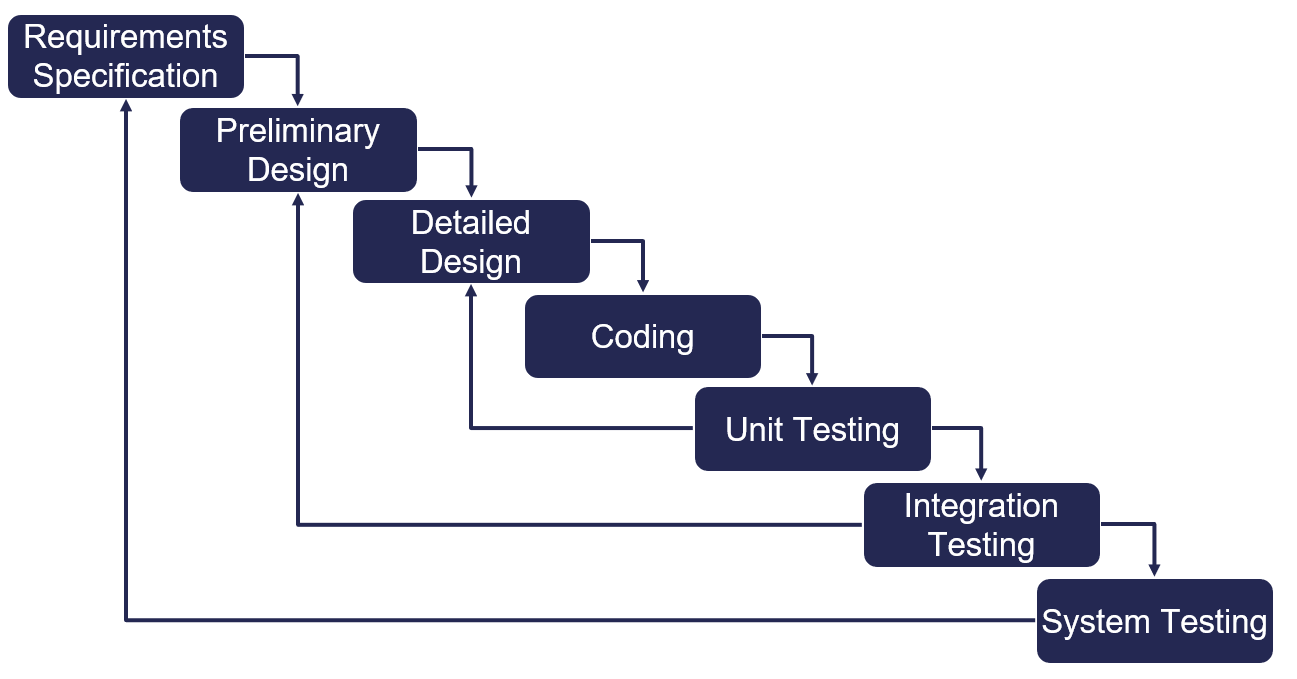
\includegraphics[width=10cm, scale=0.5]{figures/waterfall_model.png}
    \caption{The Waterfall model.}
    \label{waterfall_model}
\end{figure}

Modern software development strays away from non-incremental models, as today's applications are continuously evolving and adapting; instead, iterative approaches are preferred, where the sequential chain of the Waterfall model is replaced by a cyclical process during which the development team goes through multiple iterations or cycles of planning, designing, building, testing, and evaluating the product.

A key example is the Agile SDLC model, which values flexibility and collaboration, and prioritizes customer satisfaction and working software over strict plans and documentation. One of the main principles of Agile development is the use of small, cross-functional teams that work together to deliver working software in short iterations, or "sprints": this allows for frequent feedback and adjustments to be made throughout the development process between the clients and the development teams, rather than waiting until the end of a project to make changes.
Figure \ref{agile_model} highlights the phases of the Agile process:

\begin{figure}[h]
    \centering
    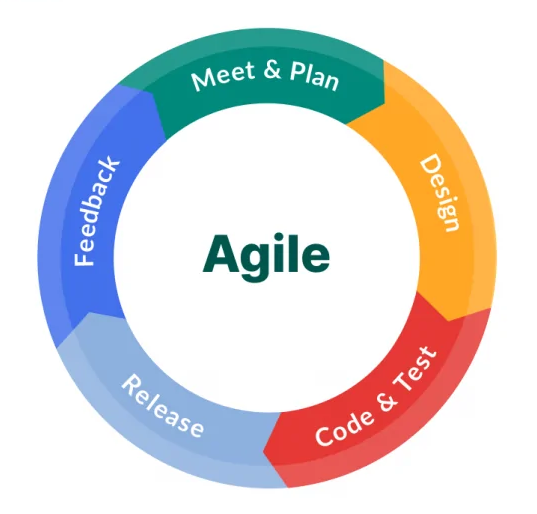
\includegraphics[width=8cm, scale=0.2]{figures/agile_model.jpg}
    \caption{The Agile model.}
    \label{agile_model}
\end{figure}

\noindent The main steps performed during each of these phases are summarized below:
\begin{itemize}
    \item \textbf{Design}: in this phase, the team designs the architecture, user interface and overall functionality of the software; the design process is iterative and collaborative, with the team working closely with customers, as well as with the stakeholders, with the objective to ensure that the software meets the agreed-upon needs.
    \item \textbf{Code \& Test}: during this phase, the team writes the code for the software and performs testing to ensure that it is functioning correctly; Agile development places a strong emphasis on automated testing, which allows for quick feedback on the quality of the delivered code modules.
    \item \textbf{Release}: the team releases the software to customers and stakeholders; this allows developers to gather feedback on the software before the final release.
    \item \textbf{Feedback}: the team reviews the feedback received from customers and stakeholders and makes any necessary changes to the software. Since this feedback is also incorporated into the development process in an iterative manner, it allows the software to continuously improve over time.
    \item \textbf{Meet \& Plan}: the team meets to plan the next iteration of development, reviews the progress made in the previous iteration, sets goals for the next one, and assigns tasks to team members. The team also reviews and adjusts the development plan as needed to ensure that the software is on track to meet the customers' needs.
\end{itemize}



\section{Test-Driven Development}
\subsection{Overview}
Unit testing is arguably the most practiced testing technique, since by itself it can already provide a general assessment of the quality and reliability of a software solution. \tdd is a software development approach that builds on top of the concept of unit testing, firstly introduced in 2003 by Kent Back in the book \textit{``Test-Driven Development By Example"} \cite{TDDByExample}; while there is no formal definition of the process, the goal is to \textit{``write clean code that works"}, as the author states. With \tdd, test cases are written before any production code: these tests are used to define the requirements for the system and to guide the development process, with the objective of this practice being for all these tests to pass before the development is complete, by continuously running the entire test suite as more features are tested and built; this can help to ensure the quality and reliability of software. Moreover, \tdd encourages software developers to write small, isolated units of code that are easy to test, maintain and understand, and will ultimately act themselves as a form of documentation for the developers. 
Compared to traditional testing and SDLC approaches, \tdd is an extremely short, incremental, and repetitive process, which make it strongly related to test-first programming concepts in Agile development and Extreme Programming; this advocates for frequent updates/releases for the software, in short cycles, while encouraging code reviews, unit testing and incremental addition of features.


At its core, \tdd is made up of three iterative phases: \textit{Red}, \textit{Green} and \textit{Blue} (or \textit{Refactor}):
\begin{itemize}
    \item In the \textbf{\textit{Red}} phase, a test case is written for the chunk of functionality to be implemented; since the corresponding logic does not exist yet, the test will obviously fail, with the source code often not even compiling.
    \item In the \textbf{\textit{Green}} phase, only the code that is strictly required to make the test pass is written.
    \item Finally, in the \textbf{\textit{Blue}} phase, the implemented code, as well as the respective test cases, is refactored and improved. It is important to perform regression testing after the refactoring to ensure that the changes did not result in any unexpected behaviors in other components.
\end{itemize}
Each new unit of code requires a repetition of this cycle \cite{GuidelinesTDD}. Figure \ref{tdd-cycle} provides a visual representation of the \tdd process.

\begin{figure}[h]
    \centering
    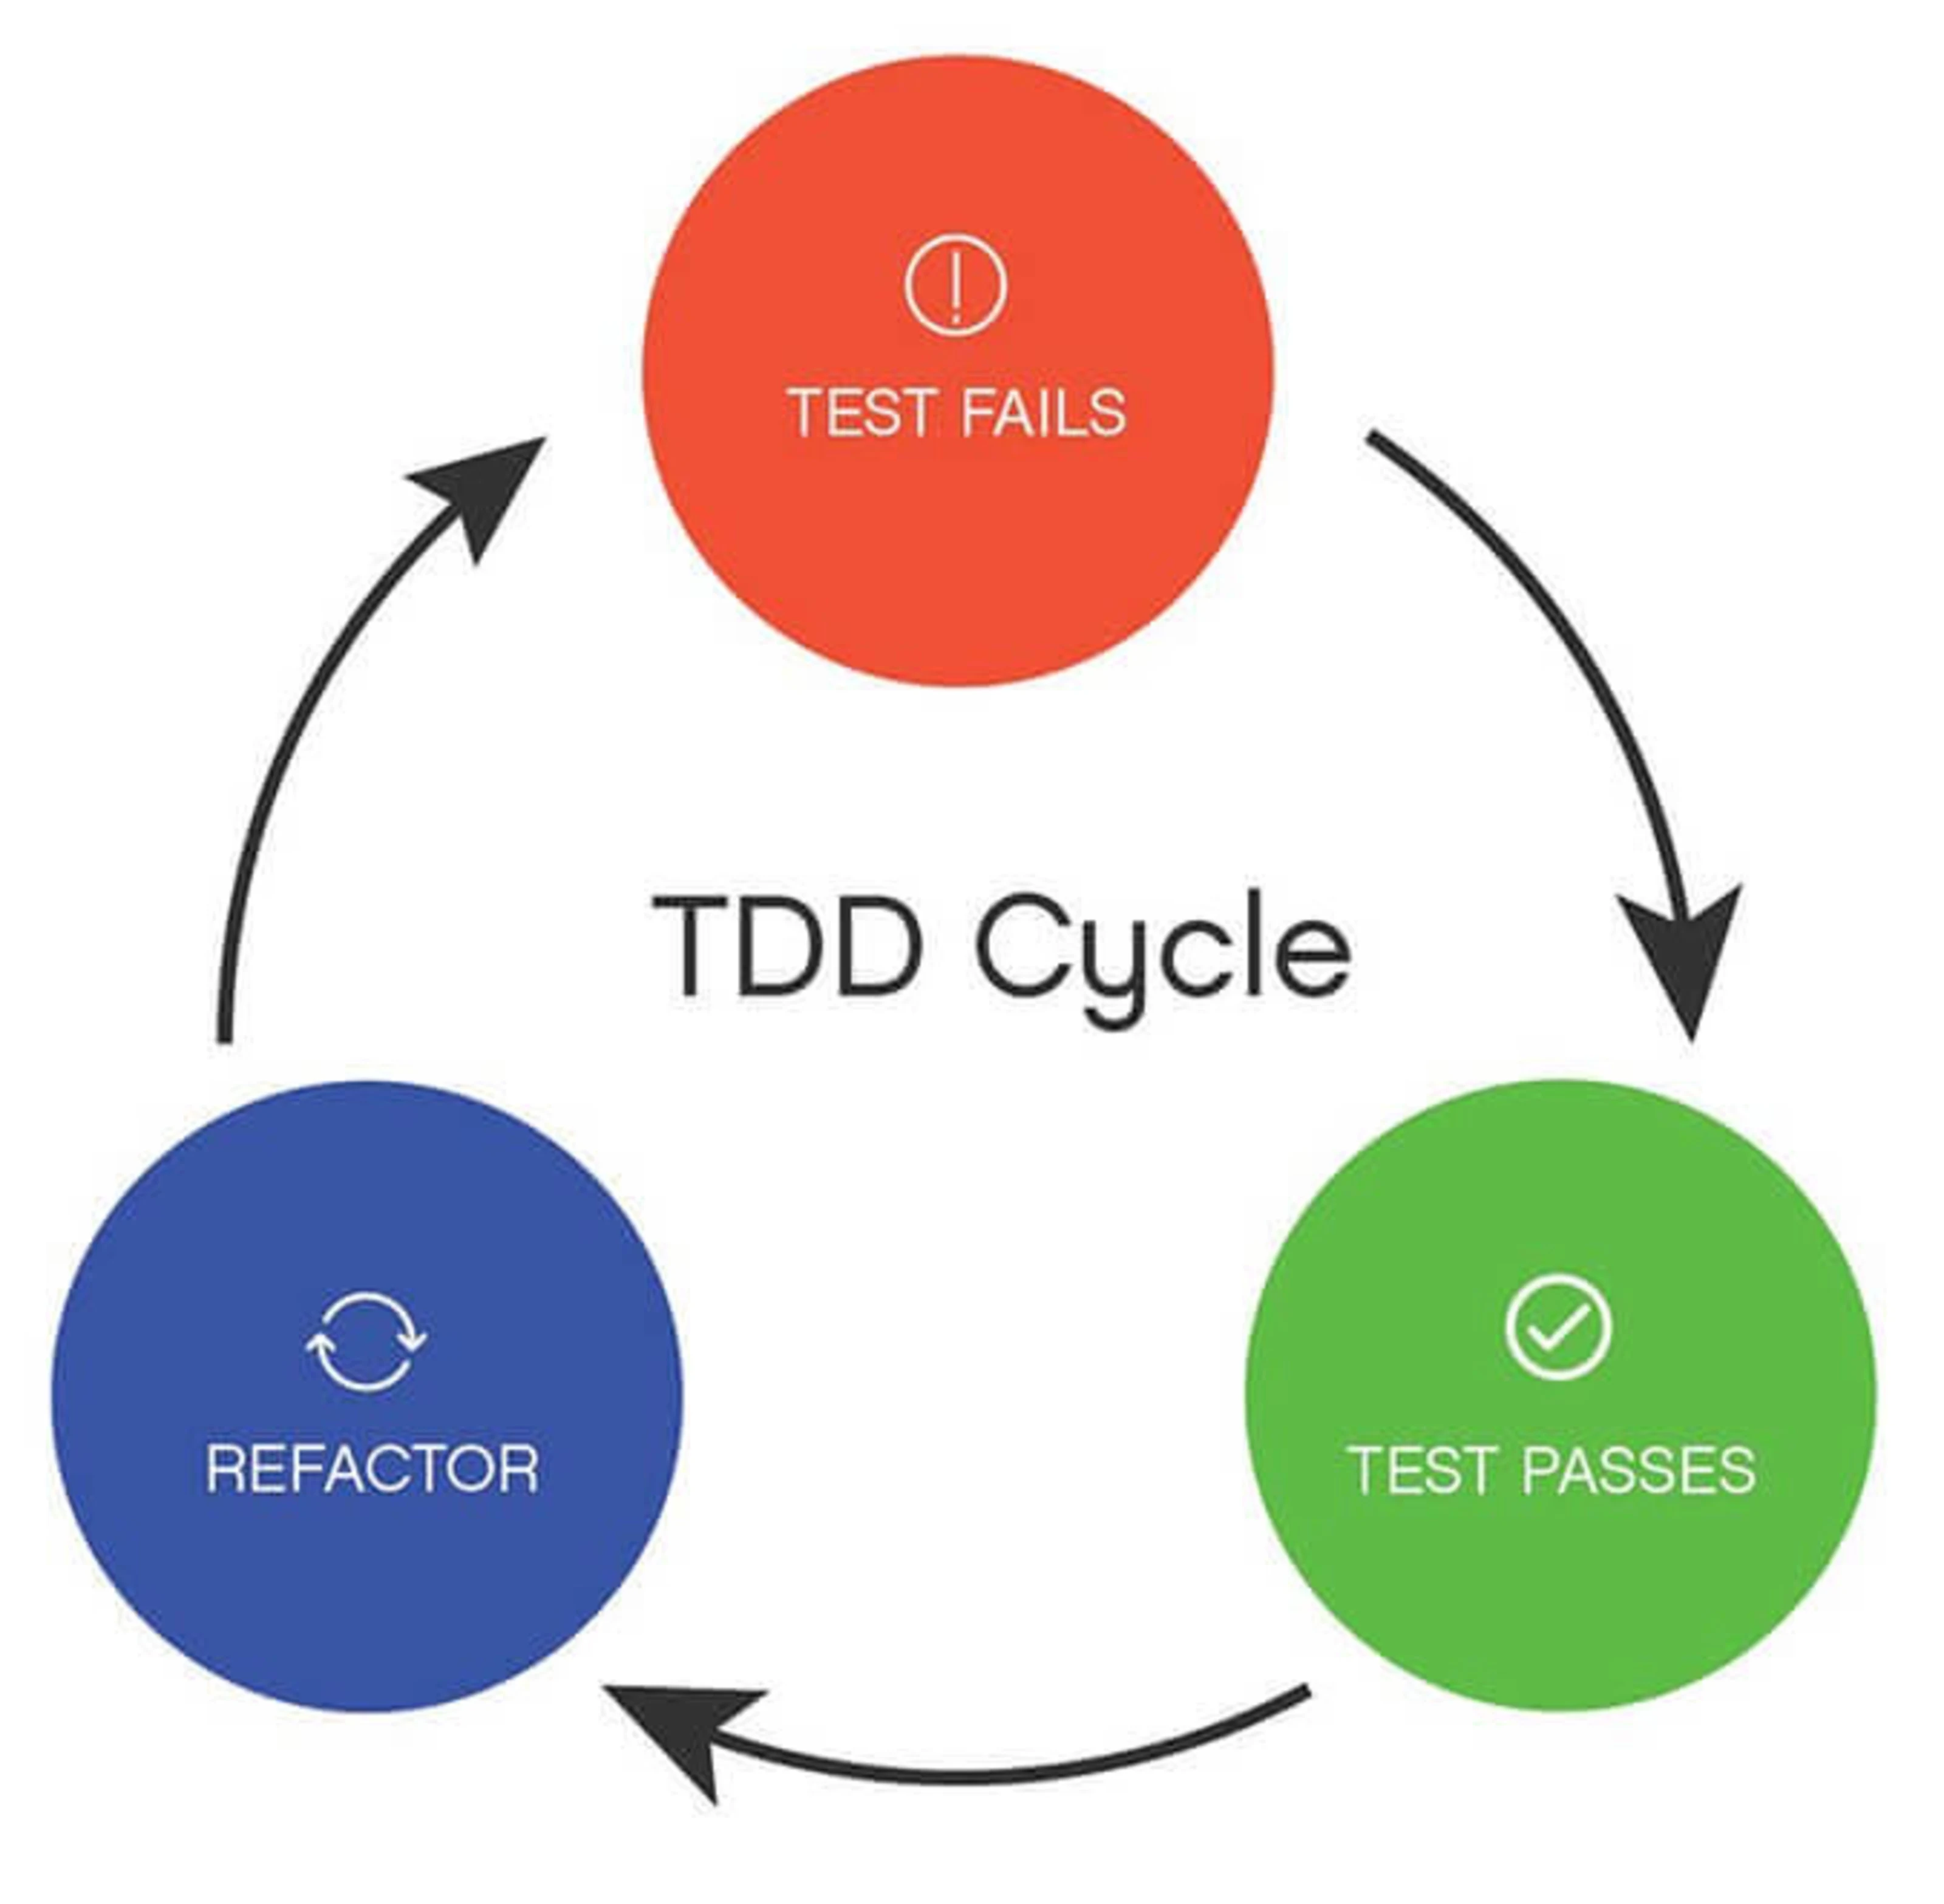
\includegraphics[width=8cm, scale=0.2]{figures/tdd_cycle.jpg}
    \caption{The Test-Driven Development cycle.}
    \label{tdd-cycle}
\end{figure}

As previously stated, each \tdd iteration should be extremely short, usually spanning from 10 to 15 minutes at most: this is possible thanks to a meticulous decomposition of the system's requirements into a set of user stories, each detailing a small chunk of a functionality specified in the requirements; these stories can then be prioritized and scheduled to achieve an iterative implementation of the system. The specification of user stories can also vary in granularity: when using a fine-grained structure to describe a task, this can be broken up into a set of sub-tasks, each corresponding to a small feature; on the other hand, with coarser-grained tasks, this division is less pronounced \cite{DBLP:journals/tse/KaracTJ21}. Even when the same task is considered, the outcome of the \tdd process will change depending on the level of granularity employed when describing it; there is no overall right or wrong approach, rather it is something that comes from the experience of the developer to break tasks into small work items \cite{DBLP:journals/tse/KaracTJ21}.


\subsection{\tdd advantages and challenges}
The employment of \tdd can result in a series of benefits during the development process, such as:
\begin{itemize}
    \item \textbf{Very high code coverage}: coverage is a metric used to determine how much of the code is being tested; it can be expressed according to different criteria such as statement coverage - \ie how many statements in the code are reached by the test cases - branch coverage - \ie how many conditional branches are executed during testing - or function coverage - \ie how many functions are called when running the test suite. While different coverage criteria result in different benefits, by employing \tdd we ensure that any segment of code written has at least one associated test case.
    \item \textbf{Improved code quality and maintainability}: as we are specifically writing code to pass the tests in place, and refactoring it after the \textit{Green} phase, we ensure that the code is cleaner and overall easier to understand, without any extra pieces of functionalities that may not be needed, leading to a more maintainable architecture in the long run.
    \item \textbf{Regression testing}: by incrementally building a test suite as the different iterations of \tdd are performed, we allow the system to always be ready for this suite to run whenever new changes or functionalities are pushed to its codebase.
    \item \textbf{Improved code readability and documentation}: well-written tests serve as documentation for the code, making it easier for new contributors to understand it.
    \item \textbf{Simplified debugging and early fault detection}: whenever a test fails it becomes obvious which component has caused the fault: by adopting this incremental approach and performing regression testing, if a test fail we will be certain that the newly written code will be responsible. For this reason, faults are detected extremely early during the testing process, rather than potentially remaining hidden until the whole test suite has been built and executed.
\end{itemize}
Similarly, however, the \tdd approach can result in a series of pitfalls and challenges:
\begin{itemize}
    \item \textbf{Learning curve}: \tdd requires a different way of thinking about software development, which can be challenging for some developers to learn.
    \item \textbf{Overhead of maintaining tests}: maintaining a comprehensive suite of tests requires time and effort, and can become a burden for developers as the codebase grows. 
    \item \textbf{False sense of security}: as with traditional testing, if tests are not comprehensive or not properly written/maintained, they can give a false sense of security about the code's quality.
    \item \textbf{Rigidity}: \tdd can lead to a rigid and inflexible code structure, as the tests dictate the core design of the application; this can limit creativity and experimentation, as developers may be reluctant to change the code if they know it will break the tests.
    \item \textbf{Difficulty in testing certain types of code}: user interfaces or performance-critical code can be challenging to test using \tdd; developers may still need to use additional testing methods or tools to ensure adequate coverage for these types of code.
    \item \textbf{Slower initial development}: writing tests before code can slow down the initial development process, as it requires additional time and effort. However, as we saw, this investment should generally pay off in the long run by reducing the need for reworks and debugging.
\end{itemize}

Keep in mind that the benefits and challenges of \tdd discussed in this section are often not based on empirical evidence.

    \chapter{Embedded Systems}
    \chapter{Embedded Systems}
\section{Overview}
\ess can be defined as a combination of hardware components and software systems that seamlessly work together to achieve a specific purpose; they can be dynamically programmed or have a fixed functionality set, and are often engineered to achieve their goal within a larger system. They are commonly found inside devices that we use on a daily basis, such as cell phones, traffic lights, and appliances; here, these systems are responsible for controlling the functions of the device, and they are required to work continuously without the need for human intervention, besides the occasional battery replacement/recharge.
This requirement implies that, in most circumstances, providing maintenance to \ess is challenging or straight up unfeasible; therefore, the design process of a system of this kind must account for a series of additional challenges and constraints, that are typically not considered as much in \noess, in order to guarantee their ability to operate in a stand-alone manner and in a wide range of conditions. Many \ess, in fact, are deployed into physical environments that do not have access to a network, are not covered by an internet connection, or are even subject to harsh and adverse weather conditions.
Furthermore, many \ess are used in applications that require a high degree of safety and security, such as in the aerospace or medical industries, meaning that there is a need for the system to operate without fail and without compromising safety. 

Despite the many challenges, in recent years, \ess have seen a steep surge in popularity, and have driven innovation forward in their respective areas of interest: everywhere, spanning from the agricultural field, to the medical and energy ones, \ess of various size and complexity are employed, especially in areas where human intervention is impractical or straight up impossible.
As the demand for more advanced and sophisticated devices continues to increase, the role of \ess will only become more prominent; the global \ess market, in fact, is expected to witness notable growth. A recent report evaluated the global \ess market 89.1 billion dollars in 2021, and this market is projected to reach 163.2 billion dollars by 2031; with a compound annual growth rate of  6.5\%~ \cite{ESSTR2022}. This growth is mostly related to  an increase in the demand for advanced driver-assistance system (in electric and hybrid vehicles) and in the number of \ess-related research and development projects. 





\section{Enabling technologies}
\subsection{Microcontrollers}
One of the key enabling technologies for \ess is their microcontroller, which is a small single-chip computer that is used to manage the functions of the larger system, in a power-efficient way and ideally at a low cost. While some applications require their own custom-made microcontroller and other custom hardware components built ad-hoc for them, there is a wide variety of general-purpose microcontroller boards, sensors, and actuators that are far easier to program and can also be customized for a high range of applications, which makes them highly versatile.

One type of general-purpose microcontroller that is commonly used for \ess development, as well as for many other Internet of Things (IoT) purposes, is the Arduino: an open-source platform that is based on the Atmel AVR microcontroller; it is widely used in hobbyist and educational projects because of its simplicity and low cost. Many Arduino versions and revisions exist, each with a different form factor, amounts of on-board resources, and I/O pins; as a result, they are used for applications of increased complexity and needs. Some examples include the Arduino Nano, with the smallest form factor among the Arduino boards and very limited, the Uno, and the Mega, with the highest amount of analog/digital pins and resources.

Another popular general-purpose microcontroller platform is the Raspberry Pi, a small single-board computer that is based on the ARM architecture, which is also what many mobile processors are based on. It comes in different variants, from an Arduino Nano-sized Raspberry Pi Zero and Zero W, but equipped with much more resources, to the Pi 3 and 4 models, which are effectively capable of running a more complex OS, supporting even up to 8GB of RAM.

In addition to these general-purpose microcontrollers, there are also many proprietary devices that are designed for specific applications: given this high specialization, these microcontrollers often offer limited customization capabilities, and may not be easily programmable, if at all, by the user. Some examples of proprietary microcontrollers include the Microchip PIC and the Texas Instruments MSP430; these chips are often used in industrial and commercial applications, where a high level of performance and reliability is required. They may also be used in applications where security is a concern, as their design may be kept confidential to protect against tampering or reverse engineering attempts.

Overall, the choice of microcontroller for an \es will depend on the specific requirements of the user. General-purpose microcontrollers such as Arduino and Raspberry Pi may be suitable for hobbyist or educational projects, while proprietary microcontrollers may be better suited for industrial or commercial applications where performance and reliability are critical.


\subsection{Embedded software and communication protocols}
Software-wise, more complex \ess can be equipped with their own \textbf{Embedded Operating System} (EOS), specifically designed to run on embedded devices, as they have a smaller footprint and fewer features compared to general-purpose OSs like Windows or Linux, and are optimized  for low power consumption. Popular EOSs include TinyOS and Embedded Linux.
Furthermore, the real-time requirements of some \ess calls for their own \textbf{Real-Time Operating System} (RTOS); these are specialized OSs that are designed to provide a predictable response time to events, even when there are many tasks running concurrently. RTOS are essential for \es that require fast and reliable performance, such as in aircraft control systems or medical devices. A notable and open-source example is FreeRTOS. 


At the lower level, communication between different components is crucial for the proper functioning of the system; there are various communication protocols that allow transmission and exchange of data, with the most notable ones being UART, I2C, and SPI:
\begin{itemize}
    \item \textbf{Universal Asynchronous Receiver/Transmitter (UART)}: one of the simplest protocols used for serial communication between devices; it is full-duplex, which means that data can be transmitted and received at the same time. UART is widely supported by many microcontrollers and microprocessor devices, however, it is typically slower than other communication protocols and can be less reliable over longer distances.
    \item \textbf{Inter-Integrated Circuit (I2C)}: a two-wire communication protocol that is used for communication between devices on the same circuit board; it is a half-duplex protocol, so data can only be transmitted or received at a time. I2C is commonly used to connect devices such as sensors, displays, and memory to a microcontroller. It is relatively fast and can support multiple devices on the same bus; however, it still has a limited data rate.
    \item \textbf{Serial Peripheral Interface (SPI)}: a two-wire communication protocol used for communication between devices; it is a synchronous protocol, which means that data is transmitted and received in a coordinated manner. SPI is relatively fast and can support multiple devices on the same bus, however, it requires more wires and pins compared to I2C and as a reseult can be more complex to implement.
\end{itemize} 


Besides communication between different components sharing the same circuit, multiple devices are often deployed as part of a larger system and must be able to efficiently communicate between each other to achieve their purpose; therefore, it is essential for \ess to be equipped with a robust suite of wireless communication protocols. As always, determining which protocol to employ depends on the constraints the system is dealing with, such as being limited to a low power consumption or being required to maintain a low-latency communication.

Zigbee is a wireless communication protocol specifically designed and built for low-power, low-data-rate applications \cite{Zigbee}; it is often used in sensors and other devices that need to communicate over short distances, such as in home automation systems or industrial control systems. Its very low power consumption makes it so ZigBee is one of the most well-suited protocols for use in devices that need to operate for long periods of time without access to a power source (\ie a quite substantial subset of \ess).
Bluetooth is another wireless protocol that is commonly used in \es which was designed for medium-range communication and is most commonly used to connect devices such as phones, tablets, and laptops to other devices, such as speakers, keyboards, or headphones. Bluetooth is a widely supported standard and is often used in applications where compatibility with a range of different devices is important; furthermore, with its low-energy variant, Bluetooth can help further optimize power consumption in devices that require it.
LoraWAN and SigFox on the other hand, are two Low-Power, Wide-Area (LPWA) communication protocol designed for IoT and machine-to-machine (M2M) applications; a typical use case is the transmission of small amounts of data over long distances, making them well-suited for use in remote monitoring systems or other applications where conventional communication methods are not practical.
For network communications, IP, and it's low energy version 6LoWPAN, are widely used protocols; they are exercised for transmitting data between devices at the network level and are a key component of the Internet.
Finally, at the application level, lightweight messaging protocols such as the Message Queue Telemetry Protocol (MQTT) are a common choice.





\section{Design challenges}
From a design and development standpoint, working with \ess can be complex, as it involves a wide range of skills and disciplines, including computer science, electrical engineering, and mechanical engineering. It is often necessary to work closely with other team members, for both the hardware and the software, to ensure that the system meets all of its requirements, functional and especially non-functional. 
In view of this, the main challenge resides in balancing the trade-offs between performance, power consumption, and cost.
For example, increasing the performance of an \es in order to accommodate a certain functionality's needs may require more power-hungry components, thus increasing the cost of the system and potentially conflicting with another requirement, according to which the device must be able to operate on a battery for long periods of time. Similarly, reducing power consumption to reach a power target may come at the expense of performance. 

Going through multiple hardware revisions in order to meet the requirements and fine-tune power and computational behavior iteratively can be extremely expensive. For this reason, as we discussed, general-purpose microprocessors should be considered in initial design phase; in most real systems however, there is the need for custom-made hardware, tailored according to the system's requirements, for security and reliability reasons.
Regardless of the microcontroller, optimization steps can be performed in most cases and involve using specialized programming languages and techniques, such as RTOSs and low-level hardware access, implementing power-saving modes and using low-power components to minimize power consumption.

Handling failures in \ess is another critical aspect to consider during their design phase: any failure should always be evident and identifiable quickly (a heart monitor should not fail quietly) \cite{MakingEmbeddedSystems}. Given the high criticality of many such systems, ensuring their dependability over the course of their lifespan is essential; \ess can be deployed in extreme conditions (\ie weather monitoring in extreme locations of the planet, satellite managements systems, devices inside the human body, and so on), where maintenance operations cannot be performed regularly, and high availability is expected. 
The dependability of an \es can be expressed in terms of:
\begin{itemize}
    \item \textbf{Maintainability}: the extent to which a system can be adapted/modified to accommodate new change requests. As \ess becomes more complex and feature-rich, it is becoming increasingly important to design them with maintainability in mind. This includes designing systems that are easy to update and repair, as well as ensuring that they can be easily replaced if necessary.
    \item \textbf{Reliability}: the extent to which a system is reliable with respect to the expected behavior. To improve reliability, \es should be designed with robust error-detection and correction mechanisms.
    \item \textbf{Availability} is the degree to which an \es is operational and accessible to its users; important for systems that are used in critical applications, such as transportation or medical equipment. To improve availability, \ess should be designed with multiple levels of redundancy and with robust fault-tolerance mechanisms. Additionally, it is important to ensure that the system is able to handle the challenges of limited bandwidth, high latency, and unreliable connectivity.
    \item \textbf{Security} refers to the ability of a system to protect against unauthorized access, modification, or destruction of data; important for systems that handle sensitive information, such as financial transactions or personal data. In order to improve security, \ess should be designed with robust encryption, security protocols, and authentication mechanisms, and should be thoroughly tested for vulnerabilities.
\end{itemize}

These dependability attributes cannot be considered individually, as there are strongly interconnected; for instance, safe system operations depend on the system being available and operating reliably in its lifespan. Furthermore, an \es can be unreliable due to its data being corrupted by an external attack or due to poor implementation. As usual, ensuring the validity of these dependability attributes in a real system, with respect to \es constraints requires trade-offs and compromises.





\section{Testing Embedded Systems}
Testing \ess poses a series of additional challenges compared to traditional systems: first, in the case of \ess that are highly integrated with a physical environment (such as with Cyber Physical Systems, CPSs), replicating the exact conditions in which the hardware will be deployed may be difficult; additionally field-testing of these systems can be unfeasible to dangerous or impractical environmental conditions (\eg a nuclear power plant, a deep-ocean station, or the human body). Secondly, given the absence of a user interface in many cases, the lack of immediate feedback makes the outcomes of the tests less observable. Moreover, resource constraints may not allow developers to fully deploy the testing infrastructure on the target hardware and thus slowing down further the process by impeding or delaying automation and regression testing. The hardware and software heterogeneity proper of \ess can also make it difficult to test them in a consistent and repeatable way. Finally, the testing of time-critical systems has to validate the correct timing behavior which means that testing the functional behavior alone is not sufficient.


\subsection{X-in-the-loop}
To mitigate some of these issues and approach \es testing in an incremental manner which allows engineers to only focus on one aspect at a time, the general testing process of \ess follows the X-in-the-loop paradigm \cite{DBLP:journals/software/GarousiFKY18}, according to which the system goes through a series of steps that simulate its behavior with an increased level of detail, before being effectively deployed on the bare hardware; subcategories in this area include Model-in-the-Loop, Software-in-the-Loop, Processor-in-the-Loop, and Hardware-in-the-Loop:
\begin{itemize}
    \item With \textbf{Model-in-the-Loop (MIL)} or \textbf{Model-Based Testing} an initial model of the hardware system is built in a simulated environment; this coarse model captures the most important features of the hardware system by using mathematical models \cite{XLoop}. As the next step, the controller module is created, and it is verified that the controller can manage the model, as per the requirements. Commonly, after the testers establish the correct behavior of the controller, its inputs and outputs are recorder, in order to be verified in the later stages of testing.
    \item With \textbf{Software-in-the-Loop (SIL)}, the algorithms that define the controller behavior are implemented in detail, and used to replace the previous controller model; the simulation is then executed with this new implementation. This step will determine whether the control logic, \ie the controller model can be actually converted to code and, perhaps more importantly, if it is hardware implementable. Here, the inputs and outputs should be logged and matched with those obtained in the previous phase; in case of any substantial differences, it may be necessary to backtrack to the MIL phase and make the necessary changes, before repeating the SIL step. On the other hand, if the performance is acceptable and falls within the acceptance threshold, we can move to the next phase.
    \item The next step is \textbf{Processor-in-the-Loop (PIL)}; here, an embedded processor, the one with which the microcontroller on the target hardware is equipped, will be simulated in detail and used to run the controller code in a closed-loop simulation. This can help determine if the chosen processor is suitable for the controller and can handle the code with its memory and computing constraints. At this point, developers have a general idea about how the embedded software will run on the hardware.
    \item Finally, \textbf{Hardware-in-the-loop (HIL)} is the step performed before deploying the \es to the actual target hardware. Here, we can run the simulated system on a real-time environment, such as SpeedGoat \cite{SpeedGoat}. The real-time system performs deterministic simulations and has physical connections to the embedded processor, \ie analog inputs and outputs, and communication interfaces, such as CAN and UDP: this can help identify issues related to the communication channels and I/O interface. HIL can be very expensive to perform and in practice it is used mostly for safety-critical applications. However, it is required by automotive and aerospace validation standards. 
\end{itemize}

After all these steps, the system can finally be deployed on the real hardware. A common environment for performing the simulation steps discussed above is Simulink \cite{Simulink}; it is a graphical modeling and simulation environment for dynamic systems based on blocks to represent different parts of a system: a block can represent a physical component, a function, or even a small system. Some notable features include: scopes and data visualizations for viewing simulation results, legacy code tool to import C and C++ code into templates and building block libraries for modeling continuous and discrete-time systems.

Figure \ref{simulink_model} ...aaa

\begin{figure}[H]
    \centering
    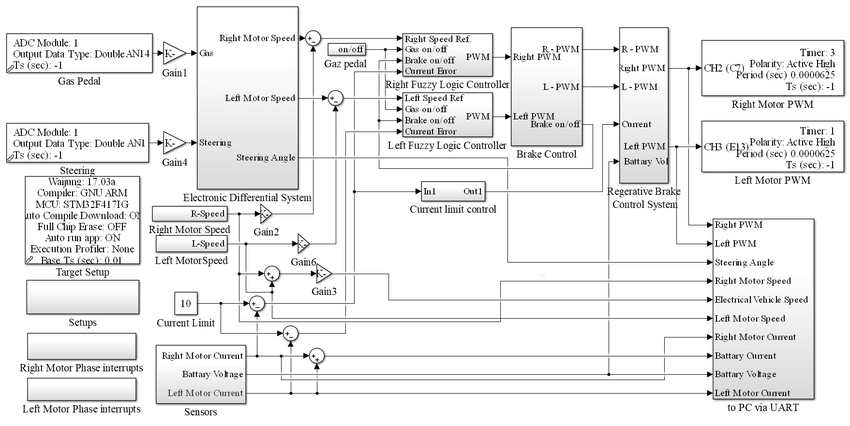
\includegraphics[width=\linewidth]{figures/simulink_model.png}
    \caption{Some components of a Simulink model for an autonomous driving system}
    \label{simulink_model}
\end{figure}


\subsection{A TDD pipeline for Embedded Systems}
Given the potential benefits of \tdd for \noess, it comes natural to ask whether this technique could be applied to the development of \ess. By applying \tdd for \ess, developers would write automated tests that would be used to verify the functionality and performance of the \es. As a reminder, these tests would be written before any code is written, and they would be used to define the requirements for the system. 
Given the higher costs of fixing issues in \ess, applying \tdd could allow developers to identify and fix problems earlier in the development process, before they become more difficult and costly to fix. It could also help to ensure that the system meets some of the requirements proper of \ess and that it is reliable, available and secure.
For the same reasons we discussed above, \tdd can be a challenging approach when applied to \ess. However, with the right tools, techniques, and experience, it is possible to apply it to \ess and to achieve the benefits of this approach. Often in fact, quality in embedded software is tied to platform-specific testing tools geared towards debugging and testing \cite{TDDEmbeddedSoftware}.
Applying TDD practices to \ess could, in theory, result in a series of benefits:
\begin{itemize}
    \item Reduce risk by verifying production code, independent of hardware, before hardware is ready or when hardware is expensive and scarce.
    \item Reduce the number of long target compile, link, and upload cycles that are executed by removing bugs on the development system.
    \item Reduce debug time on the target hardware where problems are more difficult to find and fix.
    \item Isolate hardware/software interaction issues by modeling hardware interactions in the tests.
    \item Improve software design through the decoupling of modules from each other and the hardware. Testable code is by necessity, modular.
\end{itemize}


\noindent In \cite{TDDEC}, the author proposes the "Embedded TDD Cycle", as a pipeline made of the following steps:
\begin{enumerate}
    \item \textbf{TDD micro-cycle}: this first stage is the one run most frequently, usually every few minutes. During this stage, a bulk of code is written in TDD fashion, and compiled to run on the host development system: doing so gives the developer fast feedback, not encumbered by the constraints of hardware reliability and/or availability, since there are no target compilers or lengthy upload processes. Furthermore, the development system should be a proven and stable execution environment, and usually has a richer debugging environment compared to the target platform. 
    Running the code on the development system, when it is eventually going to run in a foreign environment can be risky, so it's best to confront that risk regularly.
    \item \textbf{Compiler Compatibility Check}: periodically compile for the target environment, using the cross-compiler expected to be used for production compilations; this stage can be seen as an early warning system for any compiler incompatibilities, since it warns the developer of any porting issue, such as unavailable header files, incompatible language support, and missing language features. As a result, the written code only uses facilities available in both development environments.
    A potential issue at this stage is that in early ES development, the tool chain may not yet be decided, and this compatibility check cannot be performed: in this case, developers should take their best guess on the tool chain and compile against that compiler.
    Finally, this stage should not run with every code change; instead, a target cross-compile should take place whenever a new language feature is used, a new header file is included or a new library call is performed.
    \item \textbf{Run unit tests in an evaluation board}: compiled code could potentially run differently in the host development system and the target embedded processor. In order to mitigate this risk, developers can run the unit tests on an evaluation board; with this, any behavior differences between environments would emerge, ad since runtime libraries are usually prone to bugs \cite{TDDEC}, the risk is real. If it's late in the development cycle, and a reliable target hardware is available, this stage may appear unnecessary.
    \item \textbf{Run unit tests in the target hardware}: the objective here is again to run the test suite, however this time doing so while exercising the real hardware. One additional aspect to this stage is that developers could also run target hardware-specific tests. These tests allow developers to characterize or learn how the target hardware behaves. An additional challenge in this stage is limited memory in the target. The entire unit test suite may not fit into the target. In that case, the tests can be reorganized into separate test suites, where each suite fits in memory. This, however, does result in more complicated build automation process.
    \item \textbf{Run acceptance tests in the target hardware}: Finally, in order to make sure that the product features work, automated and manual acceptance tests are run in the target environment. Here developers have to make sure that any of the hardware-dependent code that can't be fully tested automatically is tested manually.
\end{enumerate}

    \chapter{Literature Review}
    \chapter{Literature Review}
\section{Empirical studies on Test-Driven Development}
In the past, the Empirical Software Engineering community has taken interest into the investigation of the effects of \tdd on several outcomes \cite{DBLP:conf/esem/FucciS0SSUTJO16} \cite{DBLP:journals/tse/ErdogmusMT05} \cite{DBLP:journals/infsof/Madeyski10}, including the ones of interest for this study, \ie software/functional quality and productivity. These studies are summarized in Systematic Literature Reviews (\slrs) and meta-analyses (\eg \cite{DBLP:journals/infsof/BissiNE16, DBLP:journals/infsof/MunirMP14, DBLP:journals/tse/RafiqueM13, TDDEffective}).

The \slr by Turhan \etal \cite{TDDEffective} includes 32 primary studies (2000-2009). The gathered evidence shows a moderate effect in favor of \tdd on quality, while results on productivity is inconclusive, namely there is no decisive advantage on productivity for employing \tdd. 

Bissi \etal \cite{DBLP:journals/infsof/BissiNE16} conducted another \slr that includes 27 primary studies ranging from 1999 to 2014, with the aim of locating, selecting, and evaluating available empirical studies on the application of \tdd in software development, targeting the effects that this practice produces on productivity and internal and external software quality. Similarly to Turhan \etal \cite{TDDEffective}, the authors observed an improvement of functional quality due to \tdd, while results are inconclusive for productivity. Moreover, one of the opportunities identified by this \slr for future research on the topic concerns the expansion of the \tdd practice to other paradigms and software development technologies, as most research is focused on simple examples using the \textit{Java} programming language.

Rafique and Misic \cite{DBLP:journals/tse/RafiqueM13} conducted a meta-analysis of 25 controlled experiments (2000-2011). The authors observed a small effect in favor of \tdd on functional quality, while again for productivity the results are inconclusive. 
Finally, Munir \etal \cite{DBLP:journals/infsof/MunirMP14,} in their \slr classifies 41 primary studies (2000-2011) according to the combination of their rigor and relevance. The authors found different conclusions for both functional quality and productivity in each classification.

An example of long-term investigation is the one by Marchenko \etal \cite{DBLP:conf/xpu/MarchenkoAI09}, where the authors conducted a three-year-long case study about the use of \tdd at Nokia-Siemens Network, during which they observed and interviewed eight participants (one Scrum master, one product owner, and six developers) and then ran qualitative data analyses. 
The participants perceived \tdd as important for the improvement of their code from a structural and functional perspective; furthermore, productivity increased due to the team's improved confidence with the code base. The results show that \tdd was not suitable for bug fixing, especially when bugs are difficult to reproduce (\eg when a specific environment setup is needed) or for quick experimentation due to the extra effort required for testing. The authors also reported some concerns regarding the lack of a solid architecture when applying \tdd.

Beller \etal \cite{DBLP:journals/tse/BellerGPPAZ19} executed a long-term study in-the-wild covering 594 open-source projects over the course of 2.5 years. They found that only 16 developers use \tdd more than 20\% of the time when making changes to their source code; moreover, \tdd was used in only 12\% of the projects claiming to do so, and for the majority by experienced developers.

Borle \etal \cite{DBLP:journals/ese/BorleFSGH18} conducted a retrospective analysis of a number of \textit{Java} projects, hosted on GitHub, that adopted \tdd to some extent. The authors built sets of \tdd projects that differed one another based on the extent to which \tdd was adopted within these projects; the sets of \tdd projects were then compared to control sets to determine whether \tdd had a significant impact on the following characteristics: average commit velocity, number of bug-fixing commits, number of issues, usage of continuous integration, and number of pull requests. The results did not suggest any significant impact of \tdd on the above-mentioned characteristics.

Latorre \cite{DBLP:journals/tse/Latorre14} studied the capability of 30 professional software developers of different seniority levels (junior, intermediate, and expert) to develop a complex software system by using \tdd; the study targeted the learnability of \tdd since the participants did not know that technique before participating in the study. 
The longitudinal one-month study started after giving the developers, proficient in \textit{Java} and unit testing, a training session on \tdd. After this session, the participants were able to correctly apply \tdd (\eg following the three-steps micro-cycle): they followed the \tdd cycle between 80\% and 90\% of the time, but initially, their performance depended on experience, as the seniors developers only needed a few iterations, whereas intermediates and juniors needed more time to reach a high level of conformance to \tdd. 
Experience had an impact on performance: when using \tdd, only the experts were able to be as productive as they were when applying a traditional development methodology (measured during the initial development of the system). According to the junior participants, refactoring and design decision hindered their performance. Finally, experience did not have an impact on long-term functional quality; the results show that all participants delivered functionally correct software regardless of their seniority. 
Latorre \cite{DBLP:journals/tse/Latorre14} also provides initial evidence on the retainment of \tdd: six months after the study investigating the learnability of \tdd, three developers, among those who had previously participated in that study, were asked to implement a new functionality; the results from this preliminary investigation suggest that developers retain \tdd in terms of developers' performance and conformance to \tdd.

Similarly, Romano \etal \cite{DBLP:conf/esem/Fucci0BCSTJ18} researched the retainment of \tdd knowledge and the effect on developers' productivity and external quality of software in a longitudinal study with the participation of computer science students; while their findings suggests that using \tdd does not result in a significant statistical difference on the latter constructs, employing this development practice allowed participants to write more test cases. Furthermore, this ability of novice developers to produce more tests using \tdd compared to \notdd was retained over time (6 months).

Although the above-mentioned studies have taken a longitudinal perspective when studying \tdd, none of them has mainly focused on the effect of \tdd applied to the development of \ess.


\section{Related works on embedded systems testings}
Garousi \etal \cite{DBLP:journals/infsof/GarousiFKY18} provided a systematic literature mapping for \es testing by reviewing 312 papers, concerning the types of testing activity, types of test artifacts generated, and the types of industries in which studies have focused, with the goal to identify the state-of-the-art and -practice for \ess testing.
Topics such as model-based and automated/automatic testing, test-case generation, and control systems are among the most popular ones. Most of the review papers (137 of 312, around 43.9\%) present solution proposals without rigorous empirical studies; 98 (31.4\%) papers are weak empirical studies (validation research). 36 (11.5\%) are experience papers. 34 are strong empirical studies (evaluation research). 2 and 5 papers, respectively, are philosophical and opinion papers.

In terms of level of testing considered in the papers, most of them (233 papers) considered system testing. 89 and 36 papers, respectively, focused on unit and integration testing; among the ones focused on unit testing, only two of the sources (\cite{4428578}, \cite{DBLP:conf/isese/GuanOA06}) applied \tdd to embedded software. Several practical examples of automated unit test code were provided.
The most popular technique for deriving test artifacts was requirements-based testing; 159 papers (58.4\%) discussed it. Most of these papers (142, 52.2 percent) used model-based testing, which falls into the X-in-the-loop development paradigm.
Model-based testing employs forward or backward engineering to develop models; once these models are validated, they can be used for test-case design (\eg Finite-State Machines, FSMs, and their extensions are frequently used to derive test-case sequences, employing coverage criteria such as all-transitions coverage.)
As for the type of test activities, there is a good mix of papers proposing techniques and tools for each of the test activities, with a major focus on test execution, automation and criteria-based test case design (\eg based on code coverage).
Finally, as the authors' state, there is a need for future research to conduct empirical studies providing industrial evidence on the effectiveness and efficiency of embedded software testing approaches (including \tdd) in specific contexts to further improve decision support on the selection of embedded software testing approaches beyond their SLM.



    \chapter{Experimental Approach}
    \chapter{Experimentation}
\label{chap:5_approach}
\section{Overview}
In this chapter we will present in detail the planning and approach we followed to establish the experiments on the application of \tdd for \ess, and provide an initial analysis of the results.

A controlled experiment, the baseline (\textit{Exp1}), followed by its replication (\textit{Exp2}), was conducted with the participation of 9 undergraduate final-year Master's degree and third-year Bachelor's degree Computer Science students enrolled in the \textit{Embedded Systems} course at the University of Salerno, in Italy. Participation in the studies was agreed upon by the students and was voluntary, with the outcome not directly affecting their final mark for the exam; students were however awarded 2 bonus points, in order to encourage their participation.
Before taking part in the first experiment, a set of lectures and training sessions was held with the objective of providing the participants with a common body of knowledge on the topics tackled by the experiments, namely unit testing, test scaffolding, and the \tdd approach.

Afterwards, the participants were partitioned into two groups and tackled the first task of \textit{Exp1}, one group using \tdd, the other using \notdd; this task, \textit{IntelligentOffice} (\textit{IO}) required the implementation of a system responsible for handling various parameters and functionalities inside a smart office, including the detection of workers, handling the lights and monitoring the CO2 levels inside the office.
For the second task, \textit{CleaningRobot} (\textit{CR}), the approach followed by the two groups was inverted, namely the group that implemented the first task using \tdd switched to \notdd and vice versa. This task concerned the development of an \es to manage a small cleaning robot which had to move in a room to clean dust, while avoiding obstacles along the way.
After each task of \textit{Exp1} the participants were asked to fill a questionnaire to express their feelings about the experience.

For (\textit{Exp2}), the participants had to develop an additional \es, this time at home on their own (\ie not under our supervision in a laboratory of the university), before submitting their implementation and deploying it on a real hardware platform, a \textit{Raspberry Pi Model 4}, and using real sensors and actuators. This task, \textit{SmartHome} (\textit{SH}), was focused on the implementation of an intelligent system which allowed for handling light, temperature, and gas levels inside a room.
Since \textit{Exp2} was only made up of this task, the students were randomly assigned one of the two approaches (\ie \tdd or \notdd) upon receiving the instructions for implementing this \es.
The students were given a deadline to implement the task, and were asked to book a time slot, during which they would have deployed their implementation on hardware and would have tested it in real time by observing the behavior of the sensors and actuators; moreover, each participant was individually interviewed after the hardware deployment step, in order to gather qualitative data regarding their feedback on the experiments.

Following the three tasks, we extracted the statistical values for a set of predefined dependent variables by running the acceptance test suite we prepared for each task on the implementations delivered by the participants. These values, as well as the submitted post-questionnaires and final interview, were our primary subject of analysis to answer the established research questions on the impact of \tdd on the external quality, productivity, and number of written test cases of the developers' implementations when tackling \ess.

Overall, this experimental study aims to contribute to the body of knowledge in the field of empirical software engineering by providing new insights and understanding into the application of \tdd for \es development. Furthermore, it has both research and educational goals: on one hand, we conceived the study to answer our RQs; on the other, the study allowed the participants (students) to gain practical experience with \tdd applied to \ess. As for the educational goal, \tdd is a development approach widely used in several contexts \cite{DBLP:conf/esem/RomanoZBPS22}, and it seems to be promising in the development of \ess too \cite{TDDEC}.

Although the preliminary and exploratory nature of our investigation, it has the merit to study for the first time the application of \tdd in a new development context, namely that of \ess; therefore, our results can have several practical implications, for both lecturers and researchers. For example, they could provide initial evidence on the application of \tdd to the development of \ess as to justify future research on this matter and/or promote or discourage its adoption in an industrial setting.


\newpage
\section{Research questions}
Following the main research question presented in the introduction chapter of the thesis, we defined the main goal of this study by applying the Goal/Question/Metrics (GQM) template \cite{GQM}.
According to this template, for an organization to measure purposefully it must first specify the goals for itself and its projects, then it must trace those goals to the data that are intended to define those goals operationally, and finally provide a framework for interpreting the data with respect to the stated goals.
We identify our goal as follows:

\begin{framed}
\noindent
\textbf{Analyze} the use of \tdd 
\textbf{for the purpose of} evaluating its effects in the development of \ess
\textbf{with respect to} the external quality of the implemented solution, the developers' productivity, and the number of written test cases
\textbf{from the point of} view of the researcher and lecturer 
\textbf{in the context of} an \ess course involving second year Master's degree students in Computer Science.
\end{framed}

\noindent According to this objective, the following research questions were defined:
\begin{itemize}
    \item \textbf{RQ1.} Does the use of \tdd impact the quality of the developed \es? And if so, to what extent?

    \noindent\textit{Aim}: The answer to this RQ has practical implications, especially within the Agile community: for example, in case the use of \tdd positively affects the quality of \ess developed within implementation tasks, it would mean that it is the case to teach this development approach in academic contexts, with the ultimate goal of facilitating the adoption of this Agile technique in the industry. 
    That is, if the newcomers of the working market are familiar with \tdd (because they learned and experienced it in the academic context), and it is shown that it produces \ess with improved quality, then the software industry could be encouraged to migrate their development from \notdd to \tdd.

    \item \textbf{RQ2.} Does the use of \tdd increase developers' productivity when developing \ess? And if so, to what extent?

    \noindent\textit{Aim}: A positive answer to this RQ has practical implications, since it would help us to further improve our body of knowledge in the context of \tdd applied to the development of \ess. For example, some software companies operating in the context of the development of \ess could be encouraged to use \tdd in case: \textit{(i)} there is evidence that this approach improves productivity and \textit{(ii)} developers are familiar with this approach before being hired (\eg \tdd has been learned at university).

    \item \textbf{RQ3.} Does the use of \tdd increase the number of test cases written by developers when developing \ess? And if so, to what extent?

    \noindent\textit{Aim}: If the adoption of \tdd were to result in a higher number of written test cases when developing \ess, using this approach would be beneficial to the industry. Not only more test cases would potentially cover more of the implemented source code, thus increasing reliability; additionally, the fact that tests are written as the first thing when using \tdd, a higher number of them would provide more documentation for developers and new contributors to the system, especially for those aspects of \ess that concern lower-level details, such as hardware interaction, and are generally harder to test. Finally, more tests would open up more refactoring opportunities when using \tdd; this could help with the optimization steps commonly performed in many \ess.
\end{itemize}




\section{Participants}
The participants for both \textit{Exp1} and \textit{Exp2} were Computer Science students at the University of Salerno, in Italy; they were a mix of second-year Master's degree students in Salerno, and students visiting the university by means of the Erasmus program. Both groups were enrolled in the \textit{Embedded Systems} course at the University of Salerno, however not all students had a strong Computer Science background, and among those taking the course, 9 participated. 

Participating in the studies was voluntary: the students were informed that \textit{(i)} any gathered data would be treated anonymously and shared for research purposes only; \textit{(ii)} they could drop out of the study at any time if they wished to do so, and \textit{(iii)} they could achieve the highest mark in the course even if they did not participate. Finally, as an incentive to encourage participation, those who took part in the studies were rewarded with 2 bonus points in their final mark for the course, in line with Carver \etal's advice \cite{DBLP:conf/metrics/CarverJMS03}.

Before \textit{Exp1} took place, we collected some information on the participants' knowledge and experience with general programming and testing concepts, in order to get a general idea of their personal preparation before the studies. To this end, the participants were asked to fill out a form in which they had to rate their experience using an interval-scale questions system (where 1 means “very inexperienced” and 5 means “very experienced”). All the participants had programming experience and most of them rated such an experience as 3 out of 5 on the scale. 
As for testing, the participants were mostly not experienced with unit testing, since most of them chose 1 or 2 on the scale to represent their unit-testing level of experience; finally, three students had heard about \tdd, from another university course, but none had had a practical experience with this technique before the study.

The participants for the experiments were later asked to carry out their task by either using \tdd or \notdd (\ie any approach they preferred, except for \tdd) depending on the group they were partitioned in, and on the period the task took place in. 





\section{Experimental tasks design}
The experimental objects designed for the studies are three code katas, \ie programming exercises aimed at practicing a technique or a programming language: in this case the design of a small \es, which would take around 2 hours to implement. 
All three tasks were designed according to a target platform, a \textit{Raspberry Pi Model 4}, and using the \textit{Python} programming language. As for why this environment was chosen, compared to other programming languages and platforms typically used for \ess or \iot projects (\eg \textit{Arduino} with \textit{C++}), in our opinion designing the tasks with a higher level language such as \textit{Python} - which is still employed for \ess (either in its standard form or in its \textit{MicroPython} variant), as well as for Web and Enterprise applications, as reported by IEEE Spectrum \cite{IEEESpectrum} - allowed us to focus more on the implementation and logic details than we would have done by designing the tasks orbiting around lower level language features and mechanisms.
Furthermore, if we also take into account that some participants had a limited, mostly theoretical, knowledge of \ess prior to the course's end, we think that introducing these practical concepts with \textit{Python} made it easier for them to get a grasp on the main implementation concepts for \ess. Finally, participants relied on the \textit{PyCharm IDE} to implement all three tasks, with the native \texttt{unittest} package as the testing library.

The target platform was considered even during the design of the two tasks of \textit{Exp1}, which in the end did not have to be effectively deployed on hardware; this was done in order to make the mocked implementations developed by the participants resemble as closely as possible the embedded implementations, in line with the approach proposed by Grenning \cite{TDDEC}. The main mocked component utilized was a facade for the \textit{Raspberry Pi}'s General Purpose Input/Output (GPIO) library, available as open source software on GitHub \cite{GPIOMock}. Other mocked components included third party libraries for some individual sensors and actuators, like for the \textit{DHT11} temperature and humidity sensor.
For \textit{Exp2}, another factor that influenced the design of the code kata was the availability of the hardware at the university, including sensors and actuators, as well as how hard/practical these would have been to test in real time; for example, testing a gas sensor by actually releasing gas close to it for extended periods of times could be dangerous. For some sensors, on the other hand, this was not a concern since it was possible to manually trigger them by rotating an on-board potentiometer, effectively lowering or increasing the detection threshold for their respective measurements.
The task developed for \textit{Exp2} was later deployed and tested inside a laboratory at the University of Salerno: each participant had their project uploaded on a \textit{Raspberry Pi model 4} board and assisted as we ran a small acceptance test suite in real time and logged the results (\ie which test cases passed and which failed). 

For \textit{Exp1}, the experimental tasks were:
\begin{itemize}
    \item \textbf{\textit{IntelligentOffice}} (\textbf{\textit{IO}}): task revolving around the implementation of a smart system to manage an office, by using different sensors and actuators to handle various aspects inside it. The system was responsible for detecting the presence of workers in four quadrants of the office by using infrared (IR) distance sensors, manage the light level in the room with a smart light bulb, a photoresistor (or Light Dependent Resistor, LDR), and a set of blinds controlled by a servo motor; the motor opened/closed the blinds based on the time of day and day of week measured by a Real Time Clock (RTC) module. Finally, the system would monitor the CO2 levels inside the office, with the possibility of triggering an air vent system to balance them by expelling the air outside.

    \item \textbf{\textit{CleaningRobot}} (\textbf{\textit{CR}}): as the name suggests, this task required participants to implement an \es to manage a small cleaning robot. This system received command strings from an external management unit, and had to move/rotate the robot inside the room accordingly, using two Direct Current (DC) motors, one for the wheels, and one for the robot itself. Besides this, the robot had to be able to detect obstacles in front of it by using an IR distance sensor, and had to communicate its position and the last encountered obstacle back to the remote management system after performing an action. Finally, an Intelligent Battery Sensor (IBS) was used to check the charge left of the internal battery of the robot, and a LED was turned on to signal the need for a recharge; similarly, the cleaning system of the robot would be turned on/off according to the measured remaining battery level.
\end{itemize}

As for \textit{Exp2}, the replication experiment, the \es to implement was the following:
\begin{itemize}
    \item \textbf{\textit{SmartHome}} (\textbf{\textit{SH}}): this final task concerned the development of a system which allowed the handling of light, temperature, and gas levels inside a room. By using an IR distance sensor, a photoresistor and a smart light bulb, the system managed the light level inside the room to avoid wastefully turning the light on when the user was not in the room or when it was already bright enough due to natural light. Furthermore, two temperature sensors, one on the inside and one on the outside of the room were used to collect measurements, based on which a servo motor opened or closed a window in the room. Finally, the system was also equipped with an air quality sensor to measure the gas levels inside the room; based on these measurements, in case of high amounts of gas particles detected in the air, an active buzzer would trigger an alarm to notify the user.
\end{itemize}

Further details on the experimental objects, including the list of user stories, sensors and actuators employed, and other information, are provided as an appendix to this thesis (\ref{appendix:A_IntelligengOffice}, \ref{appendix:B_CleaningRobot}, \ref{appendix:C_SmartHome}).

The material provided to the participants for each task included: \textit{(i)} a document containing the description of the task, made up of a high level description of the purpose of the system, instructions on the development approach (\ie \tdd or \notdd), and the list of user stories to implement, with each detailing the corresponding class/method to modify in the source code; and \textit{(ii)} a link to project template for the \textit{PyCharm IDE} that the participants had to import in their environment (\ie by either forking/cloning the corresponding GitHub repository or by downloading a zip file); this template contained method stubs (\ie empty methods exposing the expected API signatures), utility functions, mocked libraries for the GPIO features and other components, as well as an example empty \texttt{unittest} test class.

For each of these tasks, we prepared a corresponding acceptance test suite, as a mean to evaluate the implementations delivered by participants, and extract the metrics on which to base our empirical assessment.


\section{Study design}
The \textit{Embedded Systems} course, during which the study was conducted, started in September 2022 and covered the following topics: modeling and design of an \es, state machines, sensors and actuators, embedded processors, memory architectures, embedded security and privacy concepts, embedded operating systems and scheduling, and \ess testing techniques.

As the survey pre-\textit{Exp1} highlighted, few students had unit testing experience, and almost no participants ha dealt with \tdd up to that point: for this reason, both topics were covered through a series of frontal lectures and exercise/homework sessions in the weeks preceding the \textit{Exp1}. All the participants attended these lectures and training sessions during which they had some theoretical and hands-on experiences with the main topics they would encounter during the future experimental tasks. The overall schedule for training sessions and studies was as follows:
\begin{itemize}
    \item \textbf{Day1.} Frontal lecture - Introduction on unit testing and its guidelines - Interactive exercise on unit testing.
    \item \textbf{Day2.} Frontal lecture - Test scaffolding and \textit{Raspberry Pi}'s GPIO library - Interactive exercise on test scaffolding.
    \item \textbf{Day3.} Frontal lecture - Introduction to \tdd - Interactive exercise on \tdd.
    \item \textbf{Day4.} Training task - \tdd exercise and homework with the same structure as the future experimental task (\ie project template, a set of user stories, and 2 hours deadline).
    \item \textbf{Day6.} First task for \textit{Exp1} (\textit{IO}).
    \item \textbf{Day7.} Second task for \textit{Exp1} (\textit{CR}).
    \item \textbf{Day8.} Start date for the task relative to \textit{Exp2} (\textit{SH}).
\end{itemize}


The first task, \textit{IO} took place on Tuesday, December $6^{th}$ 2022, while the second, \textit{CR} took place on Tuesday, December $13^{th}$ 2022; both tasks required around 2 hours to be implemented by the participants. Finally, the start date for \textit{Exp2} (\ie the date when we sent out the documentation to the students) was December $19^{th}$ 2022, and the participants had to deliver their implementation by January $8^{th}$ 2023.

The design of \textit{Exp1} is an ABBA crossover \cite{DBLP:journals/tse/VegasAJ16}; it is a kind of \textit{within-participants} design where each participant receives both treatments (\ie \textit{A} and \textit{B} or, in our case, \tdd and \notdd). In ABBA crossover designs, there are two sequences (\ie \textit{G1} and \textit{G2}), defined as the order with which the treatments are administered to the participants, and two periods (\ie \textit{P1} and \textit{P2}), defined as the times at which each treatment is administered; the experimental groups correspond to the sequences. Also, to mitigate learning effects, each period is paired with a
different experimental task.

For the first period \textit{P1}, the group \textit{G1} was assigned the \tdd version of the first task, \textit{IO}, while the group \textit{G2} was assigned the \notdd version; on the other hand, during period \textit{P2}, the group \textit{G1} was assigned the \notdd version of the second task, \textit{CR}, while the group \textit{G2} was assigned the \tdd version.
Therefore, at the end of \textit{Exp1}, every participant had tackled each experimental object only once.
As for \textit{Exp2}, the group structure remained the same, however each participant was randomly assigned the \tdd or \notdd version of the third and final experimental task, \textit{SH}; specifically, 5 students ended up in the \tdd group, while 4 formed the \notdd group. As a result, the design of this study is \textit{one-factor-with-two-treatments} \cite{DBLP:books/sp/WohlinRHOR00}, a kind of \textit{between-participants} design.

After each period of \textit{Exp1}, participants were asked to fill out an online questionnaire, with the purpose of describing their general experience with the implementation of the task, focusing on their perceived complexity and testing approach. 
The structure of the post-questionnaires was made up of three interval-scale questions, and a variable number of open-ended questions, two for the \tdd group and three for the \notdd group, with the latter having an additional question, as the first open-ended one, asking to provide information about the chosen approach for testing. Furthermore, the post-questionnaire presented at the end of period \textit{P2} for \textit{Exp1} contained an additional open-ended question: here, participants had to provide their feelings towards both testing practices, \tdd and \notdd, and compare them based on the two encountered tasks. More specifically, the interval-scale questions were:

\begin{itemize}
    \item \textbf{Q1.} Regarding the comprehensibility of the provided user stories, I have found them: (Very unclear $|$ Unclear $|$ Neither clear nor unclear $|$ Clear $|$ Very clear).
    \item \textbf{Q2.} I have found the development task: (Very difficult $|$ Difficult $|$ Neither easy nor difficult $|$ Easy $|$ Very easy).
    \item \textbf{Q3.} Applying this testing approach (\ie \tdd or \notdd) to accomplish the development task has been: (Very difficult $|$ Difficult $|$ Neither easy nor difficult $|$ Easy $|$ Very easy).
\end{itemize}

\noindent As for the open-ended questions, these were:
\begin{itemize}
    \item (\textbf{\notdd only}) Describe the \notdd approach you have followed to accomplish the development task.
    \item Provide your feelings (both positive and negative) about the testing approach you used (\ie \tdd or \notdd).
    \item Provide your feelings (both positive and negative) about the development task.
    \item (\textbf{Task 2 only}) After applying the testing approach (\ie \tdd or \notdd) in the last exercise, do you have any thoughts on the differences between the two and your preference for using one over the other?
\end{itemize}

\noindent Finally, no formal questionnaire was provided for the replication study; however, after the hardware deployment and testing steps, each participant was individually interviewed about their overall experience with the studies; the structure of the final interview had a predefined script, as suggested by King \cite{King:2004}. The topics covered by the interview were:
\begin{enumerate}
    \item Provide your feelings (both positive and negative) about the final development project, (\eg development pipeline, used technologies).
    \item Provide your feelings (both positive and negative) about the development approach (\ie \tdd or \notdd) used to accomplish the final development project:
        \begin{itemize}
            \item \tdd: did you perform any refactoring? 
            \item \notdd: did you test your implementation at all? If so, which approach did you use?
        \end{itemize}
    \item Provide your feelings about the overall training experience (seminars, exercises, and homework on \tdd and \notdd, experiments, and final task):
        \begin{itemize}
            \item Positive and negative points and challenges encountered when applying TDD.
            \item What can be done to improve the application of TDD in the development of \ess?
            \item Provide a discussion on \tdd vs. \notdd in the development of \ess.
        \end{itemize}
\end{enumerate}

The answer for both the post-questionnaires and the final interviews, as well as their thematic analyses, are available as an appendix to this thesis (\ref{appendix:D_Thematic_Analysis_Baseline}, \ref{appendix:E_Thematic_Analysis_Replication}).



\section{Independent and dependent variables}
The participants were asked to carry out each task by using either \tdd or the approach they preferred (\notdd), therefore one of the independent variables considered is \textbf{\textit{Approach}}, a nominal variable assuming two values, \tdd and \notdd. The data was collected over two periods for the controlled baseline study (\textit{Exp1}), and over an additional period for the non-controlled replication study (\textit{Exp2}), so a second independent variable is \textbf{\textit{Period}}, assuming the values $P1$, $P2$, and $P3$. During the three periods both approaches (\tdd or \notdd) were applied. Finally, since the participants were split into two groups, the last independent variable is \textbf{\textit{Group}}, which can assume the values \textit{G1} and \textit{G2}.

As for the dependent variables considered in the experiments, these are: \textbf{\textit{QLTY}}, \textbf{\textit{PROD}}, \textbf{\textit{TEST}}, \textbf{\textit{CYC}}, \textbf{\textit{COG}}, \textbf{\textit{LOC}}.
The variables $QLTY$, $PROD$ and $TEST$ have been used in previous empirical studies on \noess \cite{DBLP:journals/tse/ErdogmusMT05}, \cite{DBLP:journals/tse/FucciETOJ17}, \cite{DBLP:conf/esem/Fucci0BCSTJ18}, \cite{DBLP:journals/ese/TosunDFVTESOTJJ17}. 
As for the other variables (\ie $CYC$, $COG$, and $LOC$), while they could just be used to assess constructs regarding code complexity, they can also be leveraged to further assess the quality of a software solution, since they have an impact on external attributes, such as efficiency, reliability, and maintainability.

QLTY quantifies the external quality of the solution a participant implemented. It is formally defined as follows: 
\[
    QLTY = \frac{\sum_{i=1}^{\#TUS} QLTY_i}{\#TUS} * 100 
\]
where $\#TUS$ is the number of user stories a participant tackled, while $QLTY_i$ is the external quality of the $i$-th tackled user story; to determine whether a user story was tackled or not, the asserts in the test suite corresponding to the story were checked: if at least one assert in the test suite for the story passed, than the story was considered as tackled. $\#TUS$ is formally defined as follows:
\[
    \#TUS = \sum_{i=1}^{n} 
        \begin{cases}
            1 & \text{$\#ASSERT_i(PASS) > 0$}\\
                0 & \text{otherwise}
        \end{cases}
\]
Finally, the quality of the $i$-th user story (\ie $QLTY_i$) is defined as the ratio of asserts passed for the acceptance suite of the $i$-th user story over the total number of asserts in the acceptance suite for the same story. More formally:
\[
    QLTY_i = \frac{\#ASSERT_i(PASS)}{\#ASSERT_i(ALL)}
\]
As a result, the $QLTY$ measure deliberately excludes unattempted tasks and tasks with zero success; therefore, it represents a local measure of external quality calculated over the subset of user stories that the subject attempted. $QLTY$ is a ratio measure in the range $[0, 100]$.

The PROD variable estimates the productivity of the solution implemented by a participant. It is computed as follows:
\[
    PROD = \frac{\#ASSERT(PASS)}{\#ASSERT(ALL)} * 100
\]
where $ASSERT(PASS)$ is the total number of asserts that have passed, by considering all acceptance test suites, while $ASSERT(ALL)$ refers to the total number of asserts in the acceptance suites. The $PROD$ variable can assume values between 0 and 100, where a value close to 0 indicates low productivity in the implemented solution, while a value close to 1 refers to high productivity.

The $TEST$ variable quantifies the number of unit tests a participant wrote in their implementation. It is defined as the number of assert statements in the test suite written by the participant; this variable ranges from 0 to $\infty$.

As for the additional three dependent variables, these were computed using SonarQube, an open-source platform for continuous inspection and static analysis of code \cite{SonarQube}; these variables provide additional insight regarding the quality in the implemented software solution, mostly in terms of how hard the production code is to comprehend and therefore maintain. 

They can be defined as follows:
\textbf{$CYC$} refers to the cyclomatic complexity metric of the implemented solution; it is a value used to determine the stability and level of confidence in a program, and it measures the number of linearly-independent paths inside a code module; a program with a lower cyclomatic complexity is generally easier to understand and less "risky" to modify; the variable can also be used as an estimate on how difficult the code will be to cover/test.

\textbf{$COG$} is the cognitive complexity of the solution; it is a measurement of how difficult a program module is to intuitively understand. A method's cognitive complexity is based on a few rules \cite{CognitiveComplexity}:
\begin{enumerate}
    \item Code is not considered more complex when it uses shorthand syntax that the language provides for collapsing multiple statements into one.
    \item Code is considered more complex for each break in the linear flow of the code.
    \item Code is considered more complex when flow breaking structures are nested.
\end{enumerate}

Finally, $LOC$ is the total number of lines of code written by the participant; it's defined as the sum of the individual lines of code in both the production code source files and the test code source files.

For both $CYC$ and $COG$ we only considered the production code, since there was no noticeable difference, besides one outlier, between the same metrics in the test files of the participants.

Generally speaking, the higher the values of $CYC$, $COG$, and $LOC$, the worse it is: software with high cyclomatic and cognitive complexity is more difficult to understand, maintain, and extend, and is more prone to errors and bugs. It is good practice to keep these complexities (as well as the number of lines of code, although to a lesser extent) as low as possible for easier maintenance and extensibility.





\section{Analysis methods}
\subsection{Individual analysis}
As a first way to examine the distributions of the dependent variables, we computed some descriptive statistics, for each of them. We organize this information inside a set of tables for each experimental task. Moreover, in order to provide a graphical representation of the data and to summarize the distributions, we employ box plot charts.

The information that can be extracted form a box plot chart includes:
\begin{itemize}
    \item \textbf{Minimum value}: the lowest value, excluding outliers (shown at the end of the lower whisker).
    \item \textbf{Maximum value}: the highest score, excluding outliers (shown at the end of the upper whisker).
    \item \textbf{Median}: marks the mid-point of the data and is shown by the line that divides the box into two parts. Half the values are greater than or equal to this value and half are less than this value.
    \item \textbf{Inter-quartile range}: the middle “box” represents the middle 50\% of values for the group: the range of values from lower to upper quartile is referred to as the inter-quartile range; the middle 50\% of scores fall within the inter-quartile range.
    \item \textbf{Upper quartile}: 75\% of the scores fall below the upper quartile.
    \item \textbf{Lower quartile}: 25\% of scores fall below the lower quartile.
    \item \textbf{Whiskers}: the upper and lower "whiskers" represent scores outside the middle 50\% (\ie the lower 25\% of scores and the upper 25\% of scores).
    \item \textbf{Outliers}: observations that are numerically distant from the rest of the data. They are defined as data points that are located outside the whiskers of the box plot, and are represented by a dot.
\end{itemize}



\subsection{Aggregate analysis}
Meta-analysis is a statistical method used to combine the results of multiple studies in order to obtain a more precise estimate of the effect of the treatment/intervention; its goal is to increase the power of the analysis and to provide a more robust estimate of the treatment's effects.
There are different methods used to conduct a meta-analysis, but generally, the process involves identifying the relevant studies, extracting data from them, and then analyzing this data by employing statistical techniques. 
In our case, after considering the mean, standard deviation, and number of participants for each development approach in \textit{Exp1} and \textit{Exp2}, we made use of the Standard Mean Difference (SMD) as the measure of the effect size for the meta-analysis: this value represents the difference between the two groups' mean values, standardized by dividing the difference by the standard deviation; SMD can be used to determine the overall effect size when comparing the results of the different studies. More formally, it is computed as follows:
\[
    \theta = \frac{\mu_1 - \mu_2}{\sigma}
\]
Where $\mu_1$ and $\mu_2$ represent the two means, and $\sigma$ refers to the standard deviation, used to measure the amount of variation or dispersion of a set of values.
We computed the SMD as \textit{Hedges' (adjusted) g.}; to obtain joint SMDs (one for each dependent variable), we leveraged random-effects meta-analysis models.
\noindent Based on the guidelines proposed by Cohen \cite{Cohen:1992}, the SMD can be interpreted as: \textit{negligible}, if $|\text{SMD}| <$ 0.2; \textit{small}, if 0.2 $\le |\text{SMD}| <$ 0.5; \textit{medium}, if 0.5 $\le |\text{SMD}| <$ 0.8; or \textit{large}, otherwise \cite{DBLP:conf/esem/RomanoZBPS22}.

\ \\ \
A forest plot is a common way to visually present the results of a meta-analysis: it is a representation of the effect estimates and their corresponding confidence intervals for each study included in the meta-analysis. The forest plot is divided into two parts: the left side shows the individual study results and the right side shows the overall effect estimate and its corresponding confidence interval; more specifically, the box in the middle of each horizontal line (\ie the confidence interval, CI) represents the point estimate of the effect for a single study; the size of the box is proportional to the weight of the study in relation to the pooled estimate. The diamond represents the overall effect estimate of the meta-analysis; the placement of the center of the diamond on the $x$-axis represents the point estimate, and the width of the diamond represents the 95\% CI around the point estimate of the pooled effect.



\subsection{Thematic analysis}
Thematic analysis is an approach widely used in qualitative psychology research to analyze data from interviews, focus groups, and other forms of open-ended data; this kind of analysis involves reading through the gathered unstructured data multiple times to identify recurrent patterns, concepts, or themes, and then coding these patterns using a set of codes or labels. At this point researchers would organize the coded data into themes and sub-themes, which would in turn be used to construct a narrative or a report of the findings.

Template analysis is a form of thematic analysis which emphasizes the use of hierarchical coding but balances a relatively high degree of structure in the process of analyzing textual data with the flexibility to adapt it to the needs of a particular study \cite{ThematicAnalysis}. In template analysis, it is common practice to start with some a priori themes, identified in advance as likely to be helpful and relevant to the analysis; these are always tentative, and may be redefined or removed if they do not prove to be useful for the analysis at hand. 

In our study, we used thematic analysis to analyze the open-ended questions of the post-questionnaires for the two experimental tasks of the baseline experiment, as well as the individual participant interviews of the replication study.





\section{Results}
\subsection{Dependent variable analysis}
In this section we will report the values observed for each dependent variable during their individual analysis; for each experimental task, we will provide a table summarizing the minimum and maximum values, mean, median, and standard deviation of the considered dependent variables, for the two separate approaches (\ie \tdd and \notdd), before aggregating the values of the variables for the first two tasks simultaneously, in order to provide an overview of the differences between the two testing approaches in \textit{Exp1}.
Finally, we will compare the results for both experiments, in order to provide the foundation on which to answer our research questions.
Besides the tables, we show the box plot charts to visualize the values for the statistics extracted from the dependent variables.

First, as we discussed in the dependent variables' definition section, in the end we did not take into account the cyclomatic and cognitive complexities of the test code written by the participants during the experimental tasks. 
Figure \ref{bp_task1_2_cyc_cog_test} shows the box plot chart for these metrics, relative to the experimental tasks for the baseline study:

\begin{figure}[htbp]
    \begin{subfigure}{0.5\textwidth}
        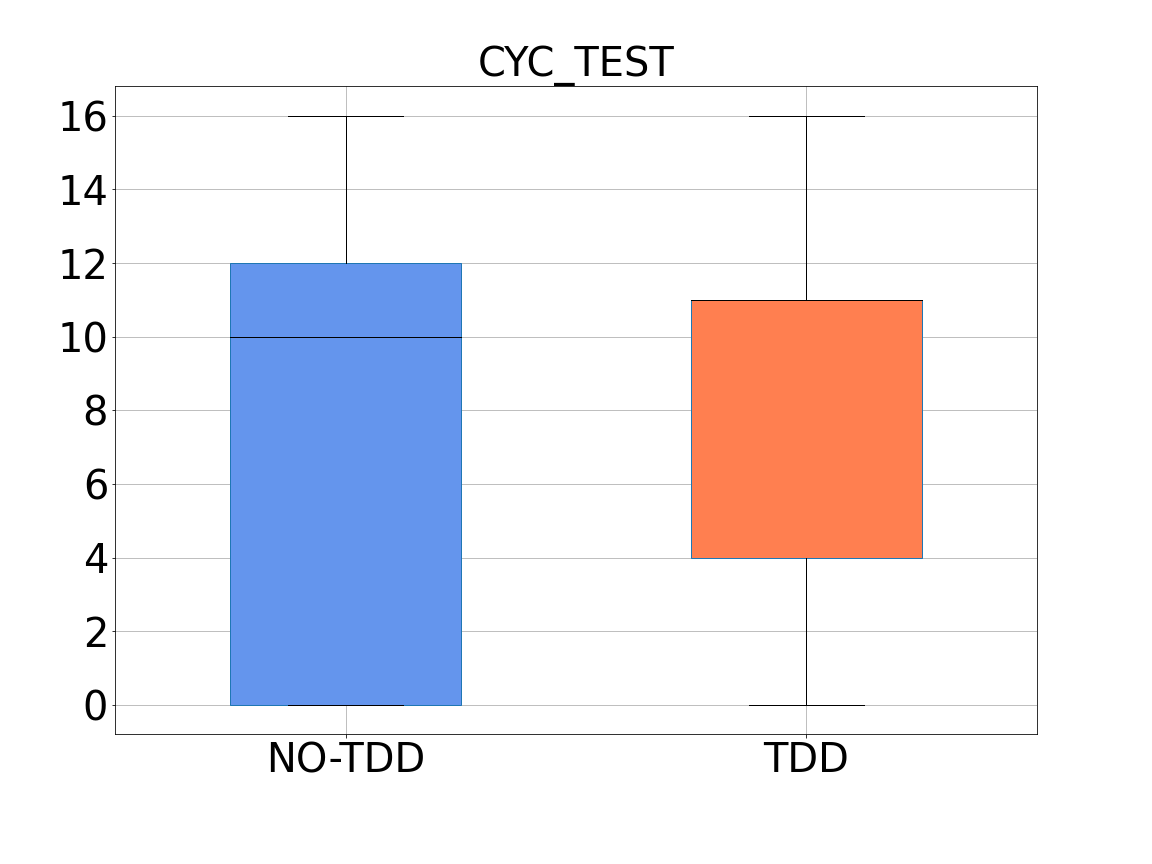
\includegraphics[width=\linewidth]{figures/box_plots/CYC_TEST.png}
        \caption{Cyclomatic complexity }
        \label{bp_task1_2_cyc_test}
    \end{subfigure}\hfil
    \begin{subfigure}{0.5\textwidth}
        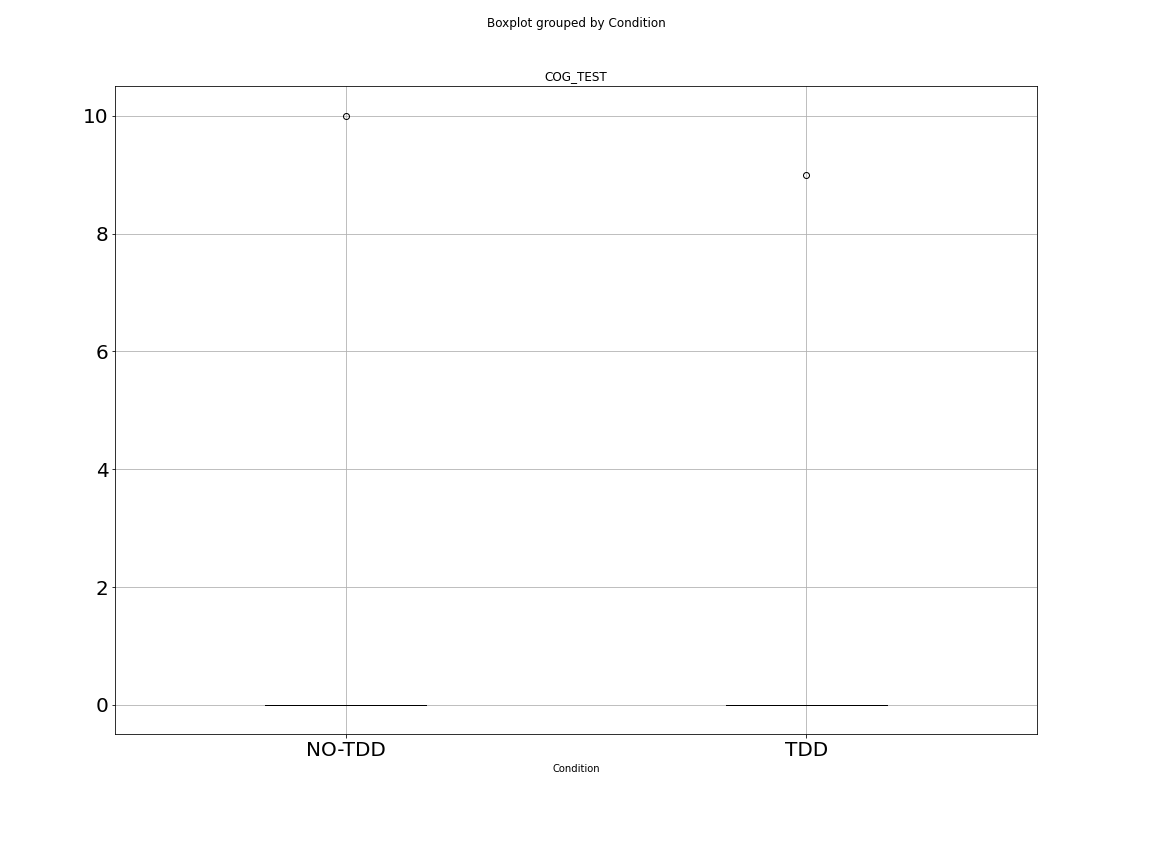
\includegraphics[width=\linewidth]{figures/box_plots/COG_TEST.png}
        \caption{Cognitive complexity}
        \label{bp_task1_2_cog_test}
    \end{subfigure}
    \caption{Box plots for the cyclomatic and cognitive complexities of test code for the first two tasks}
    \label{bp_task1_2_cyc_cog_test}
\end{figure}

Furthermore, we originally intended to also analyze the number of code smells in both the production and test code, however, as figure \ref{bp_task1_2_smells} highlights, there was no significant difference between the two approaches.

\begin{figure}[H]
    \centering
    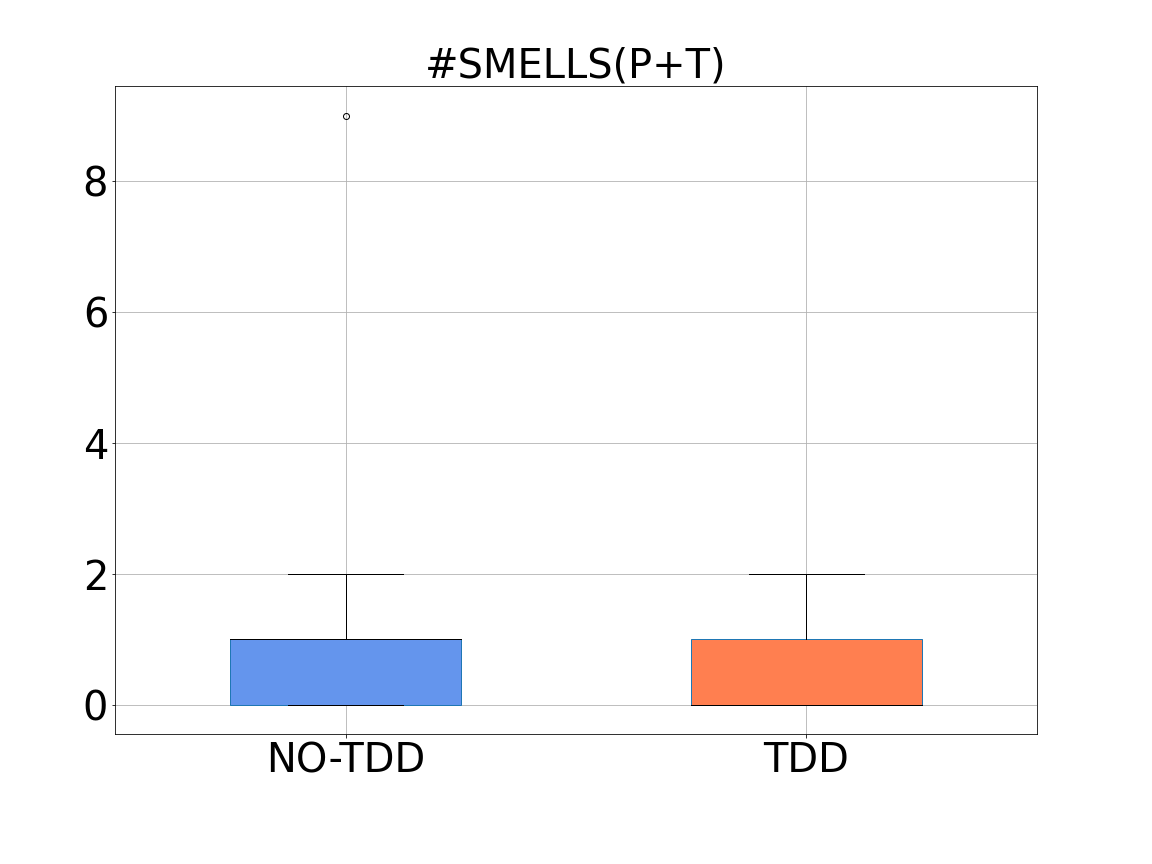
\includegraphics[width=0.5\linewidth, scale=0.5]{figures/box_plots/SMELLS.png}
    \caption{Number of code smells for the two tasks of \textit{Exp1}.}
    \label{bp_task1_2_smells}
\end{figure}


Starting with the first experimental task of \textit{Exp1}, table \ref{tab_dv_t1}, as well as figure \ref{box_plots_task1} show the tables containing the extracted statistical measures and the box plot charts for the dependent variables, respectively.

\begin{table}[H]
    \begin{center} 
        \begin{tabular}{|p{1.8cm}||p{1.6cm}|p{1.6cm}|p{1.6cm}|p{1.6cm}|p{1.6cm}|p{1.6cm}|}
            \hline
                \multicolumn{6}{|c|}{\textit{Exp1} - \textit{IO} - TDD} \\
            \hline
                Metric & Min & Max & Mean & Median & Std \\
            \hline
                QLTY & 73 & 96 & 81.12 & 77.77 & 10.73 \\
                PROD & 72 & 96 & 83 & 82 & 10 \\
                TEST & 8 & 10 & 9.5 & 10 & 1 \\
                CYC & 21 & 28 & 24.75 & 25 & 2.87 \\
                COG & 14 & 25 & 19 & 18.5 & 4.69 \\
                LOC & 154 & 195 & 167 & 159.5 & 18.95 \\
            \hline\hline
                \multicolumn{6}{|c|}{\textit{Exp1} - \textit{IO} - NO-TDD} \\
            \hline
                Metric & Min & Max & Mean & Median & Std\\
            \hline
                QLTY & 65.55 & 82 & 75.35 & 78.77 & 7.43 \\
                PROD & 56 & 84 & 76 & 80 & 11.66 \\
                TEST & 0 & 12 & 3.8 & 0 & 5.49 \\
                CYC & 12 & 18 & 15.6 & 16 & 2.19 \\
                COG & 9 & 17 & 14 & 15 & 3 \\
                LOC & 74 & 157 & 111.6 & 100 & 33.69 \\
            \hline
        \end{tabular}
        \caption{\label{tab_dv_t1}Dependent variables' statistics for task 1 of \textit{Exp1} - \textit{IO}}
    \end{center}
\end{table}

Here, $QLTY$ and $PROD$ paint the same picture, with both having a similar median and distribution of values among the two groups, with the group employing \tdd reporting slightly higher average and maximum values.
As for the number of written tests, every participant in \textit{G1} (\tdd), except for an outlier, wrote a similar number of tests (\ie 9 or 10), with a standard deviation of only 1, compared to \textit{G2}, where the number of written test cases fluctuates a lot more; still, however, the median for \textit{G2} is 0, since a few participants did not write any tests at all. Interestingly, the maximum value for $TEST$ in the \notdd group is higher than the maximum value for \tdd.
The other code quality metrics, $CYC$, $COG$, and $LOC$ are on average higher for the \tdd implementations, but still not significant (keep in mind that each function has a minimum cyclomatic complexity of 1, and the values here are considering the entire program).
A higher value of $LOC$ is generally expected for the \tdd implementation since this metric aggregates the lines of code in both the production code and the test files; however, even by considering the individual values for $LOC$ in the production and test files (not reported here), there is still not a significant difference in lines of code with respect to the implemented user stories, for both groups. We will however keep displaying the value of $LOC$ as an aggregated measurement, in order to highlight how the number of test cases impacts it.

\begin{figure}[H]
    \centering
    \begin{subfigure}{0.33\textwidth}
        \includegraphics[width=\linewidth]{figures/box_plots/task1/QLTY.png}
        \caption{QLTY}
        \label{bp_task1_qlty}
    \end{subfigure}\hfil
        \begin{subfigure}{0.33\textwidth}
        \includegraphics[width=\linewidth]{figures/box_plots/task1/PROD.png}
        \caption{PROD}
        \label{bp_task1_prod}
    \end{subfigure}\hfil
    \begin{subfigure}{0.33\textwidth}
        \includegraphics[width=\linewidth]{figures/box_plots/task1/TEST.png}
        \caption{TEST}
        \label{bp_task1_test}
    \end{subfigure}

    \medskip
    \begin{subfigure}{0.33\textwidth}
        \includegraphics[width=\linewidth]{figures/box_plots/task1/CYC.png}
        \caption{CYC}
        \label{bp_task1_cyc}
    \end{subfigure}\hfil
    \begin{subfigure}{0.33\textwidth}
        \includegraphics[width=\linewidth]{figures/box_plots/task1/COG.png}
        \caption{COG}
        \label{bp_task1_cog}
    \end{subfigure}\hfil
    \begin{subfigure}{0.33\textwidth}
        \includegraphics[width=\linewidth]{figures/box_plots/task1/LOC.png}
        \caption{LOC}
        \label{bp_task1_loc}
    \end{subfigure}
    \caption{Box plots for task 1 of \textit{Exp1} - \textit{IO}.}
    \label{box_plots_task1}
\end{figure}

In task 2 (which, as emerged from the post-questionnaires, many participants found harder compared to the previous one), the extracted statistics highlight the opposite situation (see table \ref{tab_dv_t2} and figure \ref{box_plots_task2}): while the values for $QLTY$ are still higher for the \tdd group (\textit{G2} in this case), the same thing is not true for $PROD$; this suggests that among the participants that tackled this task using \tdd, there are some that only tackled the first user stories, and did so flawlessly, thus resulting in a high value for $QLTY$ (100\% median, and 84\% mean), and a much lower value for $PROD$ (21\% median and 38.6\% mean). 
For the same reason, the average number of tests written is lower (5.4 average for \textit{G2} compared to the 9 average for \textit{G1}); the maximum value, however, is still higher for \textit{G2}, possibly resulting from a participant more extensively applying \tdd to all user stories of the task.
Finally, this time the values of $CYC$ and $COG$ are higher for the \notdd group; this is just related to the latter implementing overall more stories. The $LOC$ displays a similar behavior.


\begin{table}[H]
    \begin{center} 
        \begin{tabular}{ |p{2cm}||p{1.6cm}|p{1.6cm}|p{1.6cm}|p{1.6cm}|p{1.6cm}|}
            \hline
                \multicolumn{6}{|c|}{\textit{Exp1} - \textit{CR} - TDD} \\
            \hline
                Metric & Min & Max & Mean & Median & Std\\
            \hline
                QLTY & 50 & 100 & 84.44 & 100 & 22.70 \\
                PROD & 8 & 100 & 38.6 & 21 & 37.35 \\
                TEST & 0 & 13 & 5.4 & 3 & 5.12 \\
                CYC & 9 & 19 & 12 & 10 & 4.06 \\
                COG & 2 & 40 & 12.8 & 4.0 & 15.91 \\
                LOC & 80 & 203 & 128 & 115 & 45.61 \\
            \hline\hline
                \multicolumn{6}{|c|}{\textit{Exp1} - \textit{CR} - NO-TDD} \\
            \hline
                Metric & Min & Max & Mean & Median & Std\\
            \hline
                QLTY & 74 & 94.43 & 83.07 & 81.94 & 10.17 \\
                PROD & 52 & 73 & 60.5 & 58.5 & 10.24 \\
                TEST & 5 & 12 & 9 & 9.5 & 2.94 \\
                CYC & 16 & 36 & 23.5 & 21 & 9 \\
                COG & 11 & 49 & 29 & 28 & 15.57 \\
                LOC & 178 & 260 & 207.5 & 196 & 37.11 \\
            \hline
        \end{tabular}
        \caption{\label{tab_dv_t2}Dependent variables' statistics for task 2 of \textit{Exp1} - \textit{CR}.}
    \end{center}
\end{table}

In the task developed for \textit{Exp2}, on the other hand, (see table \ref{tab_dv_t3} and figure \ref{box_plots_task3}), we see something much more in line with the first experimental task, with results in favor of \tdd.
First, $QLTY$ and $PROD$ have a similar distribution of values for both approaches, suggesting that all stories that have been tackled are "balanced" (\ie there is no hard user story like there was in task 2); the \tdd group produced results that are around 10\% better on average.
For the number of tests, we see again a result in line with the first task, with the \tdd group producing on average many more tests, and with the minimum value for this group still well above the median of 3.5 for the \notdd group.
Regarding the three last variables associated with code complexity and quality, once again these are higher for the \tdd approach, even though, in the case of cyclomatic and cognitive complexity, the result are still not concerning from a maintainability point of view.

\begin{figure}[H]
    \centering
    \begin{subfigure}{0.33\textwidth}
        \includegraphics[width=\linewidth]{figures/box_plots/task2/QLTY.png}
        \caption{QLTY}
        \label{bp_task2_qlty}
    \end{subfigure}\hfil
        \begin{subfigure}{0.33\textwidth}
        \includegraphics[width=\linewidth]{figures/box_plots/task2/PROD.png}
        \caption{PROD}
        \label{bp_task2_prod}
    \end{subfigure}\hfil
    \begin{subfigure}{0.33\textwidth}
        \includegraphics[width=\linewidth]{figures/box_plots/task2/TEST.png}
        \caption{TEST}
        \label{bp_task2_test}
    \end{subfigure}

    \medskip
    \begin{subfigure}{0.33\textwidth}
        \includegraphics[width=\linewidth]{figures/box_plots/task2/CYC.png}
        \caption{CYC}
        \label{bp_task2_cyc}
    \end{subfigure}\hfil
    \begin{subfigure}{0.33\textwidth}
        \includegraphics[width=\linewidth]{figures/box_plots/task2/COG.png}
        \caption{COG}
        \label{bp_task2_cog}
    \end{subfigure}\hfil
    \begin{subfigure}{0.33\textwidth}
        \includegraphics[width=\linewidth]{figures/box_plots/task2/LOC.png}
        \caption{LOC}
        \label{bp_task2_loc}
    \end{subfigure}
    \caption{Box plots for task 2 of \textit{Exp1} - \textit{CR}.}
    \label{box_plots_task2}
\end{figure}

\begin{table}[H]
    \begin{center} 
        \begin{tabular}{ |p{2cm}||p{1.6cm}|p{1.6cm}|p{1.6cm}|p{1.6cm}|p{1.6cm}|}
            \hline
                \multicolumn{6}{|c|}{\textit{Exp2} - TDD} \\
            \hline
                Metric & Min & Max & Mean & Median & Std\\
            \hline
                QLTY & 85 & 100 & 95 & 100 & 7.07 \\
                PROD & 83.33 & 100 & 93.33 & 100 & 9.13 \\
                TEST & 7 & 18 & 11.6 & 12 & 4.15 \\
                CYC & 15 & 30 & 22.6 & 20 & 6.58 \\
                COG & 18 & 34 & 25.8 & 25 & 7.08 \\
                LOC & 150 & 232 & 187 & 175 & 36.15 \\
            \hline\hline
                \multicolumn{6}{|c|}{\textit{Exp2} - NO-TDD} \\
            \hline
                Metric & Min & Max & Mean & Median & Std\\
            \hline
                QLTY & 80 & 100 & 86.25 & 82.5 & 9.46 \\
                PROD & 75 & 100 & 83.33 & 79.16 & 11.78 \\
                TEST & 0 & 11 & 4.5 & 3.5 & 5.44 \\
                CYC & 16 & 23 & 19.5 & 19.5 & 2.88 \\
                COG & 19 & 25 & 21 & 20 & 2.70 \\
                LOC & 93 & 164 & 125.5 & 122.5 & 36.82 \\
            \hline
        \end{tabular}
        \caption{\label{tab_dv_t3}Dependent variables' statistics for \textit{Exp2}.}
    \end{center}
\end{table}

\begin{figure}[H]
    \centering
    \begin{subfigure}{0.33\textwidth}
        \includegraphics[width=\linewidth]{figures/box_plots/task1_2/QLTY.png}
        \caption{QLTY}
        \label{bp_task1_2_qlty}
    \end{subfigure}\hfil
        \begin{subfigure}{0.33\textwidth}
        \includegraphics[width=\linewidth]{figures/box_plots/task1_2/PROD.png}
        \caption{PROD}
        \label{bp_task1_2_prod}
    \end{subfigure}\hfil
    \begin{subfigure}{0.33\textwidth}
        \includegraphics[width=\linewidth]{figures/box_plots/task1_2/TEST.png}
        \caption{TEST}
        \label{bp_task1_2_test}
    \end{subfigure}

    \medskip
    \begin{subfigure}{0.33\textwidth}
        \includegraphics[width=\linewidth]{figures/box_plots/task1_2/CYC.png}
        \caption{CYC}
        \label{bp_task1_2_cyc}
    \end{subfigure}\hfil
    \begin{subfigure}{0.33\textwidth}
        \includegraphics[width=\linewidth]{figures/box_plots/task1_2/COG.png}
        \caption{COG}
        \label{bp_task1_2_cog}
    \end{subfigure}\hfil
    \begin{subfigure}{0.33\textwidth}
        \includegraphics[width=\linewidth]{figures/box_plots/task1_2/LOC.png}
        \caption{LOC}
        \label{bp_task1_2_loc}
    \end{subfigure}
    \caption{Aggregated box plot charts for \textit{Exp1}.}
    \label{box_plots_task1_2}
\end{figure}


\begin{figure}[htbp]
    \centering
    \begin{subfigure}{0.33\textwidth}
        \includegraphics[width=\linewidth]{figures/box_plots/task3/QLTY.png}
        \caption{QLTY}
        \label{bp_task3_qlty}
    \end{subfigure}\hfil
        \begin{subfigure}{0.33\textwidth}
        \includegraphics[width=\linewidth]{figures/box_plots/task3/PROD.png}
        \caption{PROD}
        \label{bp_task3_prod}
    \end{subfigure}\hfil
    \begin{subfigure}{0.33\textwidth}
        \includegraphics[width=\linewidth]{figures/box_plots/task3/TEST.png}
        \caption{TEST}
        \label{bp_task3_test}
    \end{subfigure}

    \medskip
    \begin{subfigure}{0.33\textwidth}
        \includegraphics[width=\linewidth]{figures/box_plots/task3/CYC.png}
        \caption{CYC}
        \label{bp_task3_cyc}
    \end{subfigure}\hfil
    \begin{subfigure}{0.33\textwidth}
        \includegraphics[width=\linewidth]{figures/box_plots/task3/COG.png}
        \caption{COG}
        \label{bp_task3_cog}
    \end{subfigure}\hfil
    \begin{subfigure}{0.33\textwidth}
        \includegraphics[width=\linewidth]{figures/box_plots/task3/LOC.png}
        \caption{LOC}
        \label{bp_task3_loc}
    \end{subfigure}
    \caption{Box plot charts for \textit{Exp2}.}
    \label{box_plots_task3}
\end{figure}

\ \\ \
Let's now consider both \textit{Exp1} and \textit{Exp2} simultaneously. As for $QLTY$, the comparison between \tdd and \notdd seems in favor of the former for any experimental task; indeed, by looking at table \ref{tab_dv_t1_2}  and figures \ref{box_plots_task1_2}.a - which aggregate the results for both tasks in \textit{Exp1} - and \ref{box_plots_task3}.a, we can notice how the boxes for \tdd in the charts are higher than, or comparable to the ones for \notdd. The same trend is confirmed by the mean and median values (see table \ref{tab_dv_t1_2}). However, we can notice that the effect of \tdd on $QLTY$ is not uniform across the experimental tasks: the gap between \tdd and \notdd is wider for the experimental task in \textit{Exp2}, while it is more limited for the two
experimental tasks in \textit{Exp1}.

As for $PROD$, it seems that the effect of \tdd is contrasting across the experimental tasks; in particular, when considering the first task in \textit{Exp1} and the one in \textit{Exp2}, the boxes for \tdd are  higher than the
boxes for \notdd (figures \ref{box_plots_task1}.b and \ref{box_plots_task3}.b). On the contrary, the box for \tdd is lower than the one for \notdd in the second experimental task of \textit{Exp1} (figures \ref{box_plots_task2}.b and \ref{box_plots_task3}.b). Such a contrasting trend is confirmed when looking at the mean and median values (see table \ref{tab_dv_t1_2}).

Finally, if we consider the number of test cases written by the participants (\ie the $TEST$ dependent variable), we can see how - similarly to the $QLTY$ variable  (see figures \ref{box_plots_task1_2}.c and \ref{box_plots_task3}.c) - the boxes for \tdd are either higher than or comparable to the ones for \notdd. Moreover, the median values for both experiments are still higher for \tdd, while the majority of values in the boxes are close together, especially in \textit{Exp2}.


\begin{table}[H]
    \begin{center} 
        \begin{tabular}{ |p{2cm}||p{1.6cm}|p{1.6cm}|p{1.6cm}|p{1.6cm}|p{1.6cm}|}
            \hline
                \multicolumn{6}{|c|}{\textit{Exp1} - TDD} \\
            \hline
                Metric & Min & Max & Mean & Median & Std\\
            \hline
                QLTY & 50 & 100 & 82.97 & 82 & 17.43 \\
                PROD & 8 & 100 & 58.33 & 72 & 35.76 \\
                TEST & 0 & 13 & 7.22 & 8 & 4.26 \\
                CYC & 9 & 28 & 17.66 & 19 & 7.51 \\
                COG & 2 & 40 & 15.55 & 14 & 12.06 \\
                LOC & 80 & 203 & 145.33 & 154 & 39.97 \\
            \hline\hline
                \multicolumn{6}{|c|}{\textit{Exp1} - NO-TDD} \\
            \hline
                Metric & Min & Max & Mean & Median & Std\\
            \hline
                QLTY & 65.55 & 94.43 & 78.78 & 78.77 & 9.11 \\
                PROD & 52 & 84 & 69.11 & 73 & 13.22 \\
                TEST & 0 & 12 & 6.11 & 7.0 & 5.08 \\
                CYC & 12 & 36 & 19.11 & 16 & 7.07 \\
                COG & 9 & 49 & 20.66 & 15 & 12.56 \\
                LOC & 74 & 260 & 154.22 & 157 & 60.32 \\
            \hline
            \hline
                \multicolumn{6}{|c|}{\textit{Exp2} - TDD} \\
            \hline
                Metric & Min & Max & Mean & Median & Std\\
            \hline
                QLTY & 85 & 100 & 95 & 100 & 7.07 \\
                PROD & 83.33 & 100 & 93.33 & 100 & 9.13 \\
                TEST & 7 & 18 & 11.6 & 12 & 4.15 \\
                CYC & 15 & 30 & 22.6 & 20 & 6.58 \\
                COG & 18 & 34 & 25.8 & 25 & 7.08 \\
                LOC & 150 & 232 & 187 & 175 & 36.15 \\
            \hline\hline
                \multicolumn{6}{|c|}{\textit{Exp2} - NO-TDD} \\
            \hline
                Metric & Min & Max & Mean & Median & Std\\
            \hline
                QLTY & 80 & 100 & 86.25 & 82.5 & 9.46 \\
                PROD & 75 & 100 & 83.33 & 79.16 & 11.78 \\
                TEST & 0 & 11 & 4.5 & 3.5 & 5.44 \\
                CYC & 16 & 23 & 19.5 & 19.5 & 2.88 \\
                COG & 19 & 25 & 21 & 20 & 2.70 \\
                LOC & 93 & 164 & 125.5 & 122.5 & 36.82 \\
            \hline
        \end{tabular}
        \caption{\label{tab_dv_t1_2}Dependent variables' statistics for \textit{Exp1} and \textit{Exp2}.}
    \end{center}
\end{table}



\subsection{Meta-analysis}
Figure \ref{fp_qlty_prod} displays the results of the aggregate analysis on the variables for \textit{Exp1} and \textit{Exp2} through means of forest plot charts, focusing on the $QLTY$ and $PROD$ variables.
The SMDs relative to the $QLTY$ variable for the single experiments (see figure \ref{fp_qlty_prod}.a) are both in favor of \tdd; in particular, the SMD is considered small (0.290) in \textit{Exp1} and large (0.950) in \textit{Exp2}, highlighting how the effect of \tdd on $QLTY$ is not uniform and may depend on the tackled task; the overall SMD is still in favor of \tdd and small (0.480).

\begin{figure}[H]
    \begin{subfigure}{0.49\textwidth}
        \includegraphics[width=\linewidth]{figures/forest_plots/QLTY.png}
        \caption{QLTY}
        \label{fp_qlty}
    \end{subfigure}\hfil
    \begin{subfigure}{0.49\textwidth}
        \includegraphics[width=\linewidth]{figures/forest_plots/PROD.png}
        \caption{PROD}
        \label{fp_prod}
    \end{subfigure}
    \caption{Forest plot charts for the $QLTY$ and $PROD$ variables.}
    \label{fp_qlty_prod}
\end{figure}

Figure \ref{fp_qlty_prod}.b displays the forest plot for the $PROD$ variable. Here, the SMD for \textit{Exp1} is in favor of \notdd and small (-0.380); this is due to the second experimental task, as expected from looking at the box plots charts in figure \ref{box_plots_task2}. For \textit{Exp2}, on the other hand, the SMD is in favor of \tdd and large (0.860). The joint SMD is still in favor of \tdd but is negligible (0.120); the hollow joint SMD indicates a higher heterogeneity ($I^2$ is more than 50\%).

Finally, figure \ref{fp_test} plots the results for the meta-analysis relative to the $TEST$ variable. Here, similarly to what happens with the $QLTY$ variable, both experiments are in favor of \tdd: the SMD for \textit{Exp1} is small (0.230), which is again expected given the contrast between the first two experimental tasks, while the SMD for \textit{Exp2} is large (1.330). The joint SMD is still in favor of \tdd and medium (0.600).

\begin{figure}[H]
    \includegraphics[width=\linewidth]{figures/forest_plots/TEST.png}
    \caption{Forest plot chart for the $TEST$ variable.}
    \label{fp_test}
\end{figure}\hfil
    
Given that for all three variables, the 95\% CI interval contains the 0, and especially considering the small size of this study, the meta-analysis alone does not indicate a statistical significance in favor of any of the two approaches for any of these variables.
A non-significant result does not mean that the treatment has no effect or that the difference is not meaningful; it simply means that there is not enough evidence to support a claim of a significant effect; therefore, we are in need of further replication to reach a statistical conclusion on the effects of \tdd on external quality, productivity, and number of tests.



\subsection{Post-questionnaire analysis}
Figure \ref{bar_charts} summarizes the answers provided by the participants in the post-experiment questionnaires submitted at the end of each task for \textit{Exp1}, comparing the responses by the employed approach (\tdd or \notdd).
Regarding user story comprehensibility, in the first experimental task, \textit{IO}, the participants had a similar level of agreement on the matter, with the majority finding the provided user stories easy or very easy. In the second task, \textit{CR}, there is a more substantial difference, with only 40\% of the \tdd group having a positive perception of the user stories' clarity, compared to the 87\% of the \notdd group.

As for the second question, regarding the feelings of the participants on the general task difficulty, in the first experimental task the participants somewhat agree, with 50\% of the \tdd group and 40\% of the \notdd group feeling neutral about the difficulty of the task; no one in the \tdd group found the task very easy, however, compared to a 20\% in the \notdd group. In the second task, the answers are quite in favor of \notdd, with 60\% of the \tdd group having some difficulties with the implementation of the provided user stories; 20\% however found the task very easy. On the other hand, all of the participants in the \notdd group agreed on feeling neutral about their ease in developing the task.

Finally, question three was focused on the difficulty of the participants in applying their reference condition: for task 1, the \tdd group did not have a strong opinion on applying this technique, with 75\% feeling neutral about it, and the other 25\% finding the application of \tdd easy but not too easy; as for the \notdd group, this had also the majority of opinions feeling neutral about their approach (60\%), however this time 20\% of the participants felt very good about applying \notdd; this is probably due to them being overall more accustomed to the approach. This conveys the idea that \tdd was considered less easy to apply compared to \notdd; such a trend is even clearer when considering the second experimental task, where 80\% of the \tdd group had trouble with their approach(40\% answered "Very Hard" and 40\% answered "Hard"), compared to only 25\% for the participants that used \notdd.


\begin{figure}[htbp]
    \begin{subfigure}{\textwidth}
        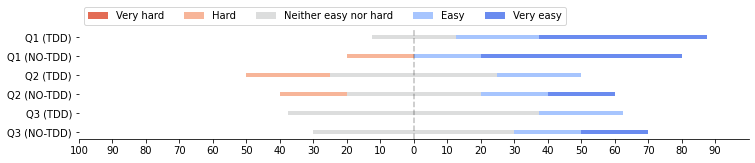
\includegraphics[width=\textwidth]{figures/bar_charts/task1.png}
        \caption{First task for \textit{Exp1}, \textit{IO}.}
    \end{subfigure}
    
    \bigskip
    
    \begin{subfigure}{\textwidth}
        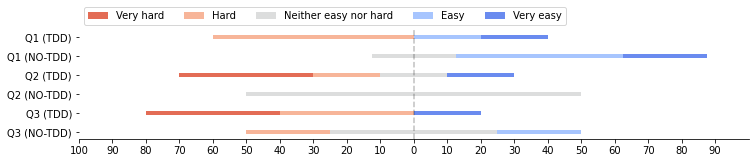
\includegraphics[width=\textwidth]{figures/bar_charts/task2.png}
        \caption{Second task for \textit{Exp1}, \textit{CR}.}
    \end{subfigure}
    
    \caption{Diverging stacked bar charts for the post-questionnaires.}
    \label{bar_charts}
\end{figure}

\newpage
Moving to the open-ended questions, we performed thematic analysis in order to identify a base template on which to parse the answers provided by the participants in the same post-questionnaires.
The themes we identified are:

\begin{enumerate}
    \item General feelings on the development task.
    \item Feelings on \tdd and \notdd to accomplish the task.
    \item \notdd testing approach.
    \item Personal comparison and thoughts between \tdd and \notdd.
\end{enumerate}

Most of the participants found the first development task easy, with 6 out of 9 expressing a positive feeling about it; 2 out of the remaining 3 found some challenges and would have liked a bit more time, while the last participant did not answer. 
For the second task, 2 out of 9 students had no issues with it, while 6 found the task to be harder than the previous one: out of the latter, 3 reported struggling with implementing some user stories, while the other 3 simply stated that the task was more challenging, without voicing in detail their struggles with it.


Employing \tdd to tackle the tasks was still not fully clear at the end of \textit{Exp1}: for task 1, 2 participants expressed how getting into the \tdd mindset for a new problem was not so easy for them, while another student, participant 2, found this practice very useful and expressed their good feelings for having learned it:
\begin{mdframed}
    \textit{``I think TDD is very helpful, and I am glad that I can learn it."}
\end{mdframed}


In the second task, which as we have seen in the interval-scale questions was considered overall harder, 3 out of 5 participants in the \tdd group expressed having trouble with it.
For example, participants 5 stated:
\begin{mdframed}
    \textit{``I think the CleaningRobot was harder than the IntelligentOffice, but maybe only because of \tdd."}
\end{mdframed}

While expressing a similar feeling, participant 8 also said how more experience with \tdd would be beneficial to them:
\begin{mdframed}
    \textit{``It is hard to think the other way around as a software developer, but I think in my opinion \tdd is very useful and if you are used to it, it can really help you a lot to improve your programming."}
\end{mdframed}

Out of the \notdd group, on the other hand, the majority had no particular issue with the approach in both tasks.
However, in the post-questionnaire for \textit{CR} 2 participants expressed how in their opinion, since this task was harder, maybe employing \tdd would have made it easier, since it would have allowed them to tackle the user stories in a more incremental manner; for example, participant 3 said:
\begin{mdframed}
    \textit{``With \tdd I wouldn't have fallen into some pitfalls; I had to rewrite some code because I didn't know I broke some components with features that I added later. With \tdd I would have known way earlier."}
\end{mdframed}

As for the chosen \notdd approach, in the first task, 3 out 5 participants dealing with this testing approach still wrote test cases after the production code, while the other 2 chose not to; for the second task, all 4 participants in the \notdd group tested their implementation, which is in line with them finding \textit{CR} overall harder.

At the end of the second task, 4 participants expressed their preference with \tdd, while 3 were still more comfortable with \notdd. Finally, one participant stated how in their opinion the best approach to use depends on how refined the requirements for the task to implement are, stating how they would prefer \tdd, but only if the functional requirements are clear, while for discovering new technologies, they wouldn't use \tdd for sure:
\begin{mdframed}
    \textit{``\tdd reduces bugs, if you break something with a refactoring you know it instantly, and the tests are like documentation. With \notdd bugs and functional errors are only known at the end of the testing phase, which for me is terrible. I would now prefer \tdd, but only if the functional requirements are clear. For discovering technology, I wouldn't use \tdd for sure."}
\end{mdframed}



\subsection{Final interview analysis}
Thematic analysis was also used to extract patterns from the final individual participant interviews; we identified the following main topics: 
\begin{enumerate}
    \item Thoughts on the replication experiment.
    \item Refactoring with \tdd.
    \item \notdd testing approach.
    \item Applying \tdd for \ess development.
    \item Prior participant testing experience.
    \item Thoughts on the overall experience with the studies, from the lectures and homework, to the last development task.
\end{enumerate}

For the first point, 5 out of 9 participants found the task straight forward and had no issues with its development, while the other 4 found it balanced, with some user stories requiring more thought before being implemented, according to them. Furthermore, 3 participants stated how they were already familiar with some of the sensors and actuators used for the task, either from previous university courses, or from personal experience.

As a reminder, for \textit{Exp2}, 5 out of 9 participants were (randomly) assigned the \tdd version, while the other 4 had to develop the \es using \notdd; out of the 5 that used \tdd, 4 of them performed some minor refactoring, either in the test cases or in the production code, while 1 did not.
As for the \notdd group, half still wrote tests (although many less compared to the \tdd group, as we have seen from the gathered data) after implementing the user stories, while the other half did not.

When discussing the employment of \tdd and \notdd in the context of \ess and their strengths and weaknesses, some participants expressed how they were not comfortable providing a definitive answer on the matter, mostly given their still limited experience with \tdd. Others conveyed how the best approach depends on the task they are working on, similarly to what happened in the post-questionnaire for \textit{CR}; for example, participant 7 said:
\begin{mdframed}
    \textit{``The task (SR) was pretty easy for me; as a result I think that \tdd was not really needed [...], it was a bit overkill. On the second task (CR), however, which I found much more complex, I feel like TDD was much more beneficial."}
\end{mdframed}

Participants also provided information about their testing experience prior to the study: 2 of them had no testing experience at all; on the other hand, 4 students already had some unit testing experience, while 3 had limited and mostly theoretical knowledge of \tdd, obtained in a previous university course.
Concerning the learning experience with \tdd, while some participants expressed how at the end of the study they were still more comfortable using \notdd, one of the students among those with no prior testing, experience stated:
\begin{mdframed}
\textit{``I had no prior testing experience at all, so it was very nice to learn about it in the lectures, especially \tdd; I would use \tdd for sure going forward, especially with even more experience. The main challenge was getting into it in the beginning."}
\end{mdframed}

Considering the last point, most students appreciated the overall experience and expressed how they enjoyed the mixture of theory and practice on \tdd and the other concepts explored. For example, participant 4 (\tdd) stated:
\begin{mdframed}
    \textit{``I enjoyed the overall experience made up of a mix of theory and practical stuff."}
\end{mdframed}

Something very interesting that came up during the thematic analysis of these interviews, especially from the lecturer's point of view, is that participants expressed a high interest into the hardware deployment step: 5 out of the 9 students that have been interviewed, in fact, demonstrated genuine interest in seeing their developed \es in action, making use of real sensors and actuators and operating on a real hardware platform. 
Participants 2 and 3, for example, stated:
\begin{mdframed}
    \textit{``Nice to see it run and test by yourself with hardware and with the sensors."}
\end{mdframed}
\begin{mdframed}
    \textit{``I knew most of the sensors so developing this task was not hard for me, but still really cool to implement because I wanted to see it in action on real hardware."}
\end{mdframed}

Keep in mind that there was no reference to this aspect in the script for the interview, so each of the participants that showed interest in the topic, did so out of their initiative while discussing their thoughts on this task; also, each student was alone during their interview, so it is unlikely that the answers were influenced by each other.




    \chapter{Discussion}
    In this section we will discuss the obtained results and the implications of this study, as well as provide an answer to the RQs and analyze potential threats to its validity.

\section{Answers to Research Questions}



\section{Implications}



\section{Threats to Validity}
According to Campbell and Stanley \cite{ResearchOfTeaching}, threats to validity are either internal or external. Internal validity concerns "controlling" the aspects of the experiment's setting to ensure that the outcomes are caused only by the introduced techniques \cite{DBLP:conf/icse/SiegmundSA15}. External validity refers to showing a real-world effect, but without knowing which factors actually caused the observed difference \cite{DBLP:conf/icse/SiegmundSA15}.
Cook and Campbell extended the list of validity categories to: conclusion, internal, construct, and external validity \cite{QuasiExp}. The latter classification has often been adopted in past empirical software engineering studies \cite{DBLP:books/sp/WohlinRHOR00}. 


In order to determine the potential threats to validity that may affect our studies, we referenced Wohlin \etal 's guidelines \cite{DBLP:books/sp/WohlinRHOR00}:
\begin{enumerate}
    \item \textbf{Internal validity} refers to the extent to which we can be confident that a cause-and-effect relationship established in a study cannot be explained by other factors; it makes the conclusions of a causal relationship credible and trustworthy. Without high internal validity, an experiment cannot demonstrate a causal link between two variables.
    There are three necessary conditions for internal validity and all three must occur to experimentally establish causality between an independent variable A (treatment variable) and dependent variable B (response variable): \textit{(i)}: the treatment and response variables change together; \textit{(ii)}: the treatment precedes changes in the response variables, and \textit{(iii)}: no confounding or extraneous factors can explain the results of the study.
    Threats to internal validity include: 
    \begin{itemize}
        \item \textbf{Deficiency of treatment setup}: the treatment setup is sometimes not appropriate, which may impact the results. For example, noise and tool performance could impact the results of a study, when they are not related to the treatment of the study.
        \item \textbf{Ignoring relevant factors}: factors not considered in the experiment setup sometimes impact the study results, such as the usability of the tools used in the experiment and their performance.
        \item \textbf{History}: A study composed of a set of treatments applied at different occasions may be impacted by the history threat. Treatments may be given to the same object at several occasions, each of which is associated with specific circumstances, such as time and location. The change in circumstances may impact the results.
        \item \textbf{Maturation:} the subjects may react differently as time passes while they perform the treatment: some may become bored and others may become motivated.
        \item \textbf{Testing}: the subjects may behave differently towards the treatment if they do it several times: they may learn the results and adapt their responses accordingly.
        \item \textbf{Treatment design}: the artifacts used in the treatment, such as the data collection form and the documents used as information source, could affect the results if not well-designed and tested.
        \item \textbf{Subject selection}: subjects for studies are selected to represent a population. The selection method affects the results and their interpretation. The group of subjects that participate in a study is always heterogeneous. The difference between individuals should not be the dominant factor for the study results: the treatment should be the dominant factor.
        \item \textbf{Sample selection}: data is usually collected from data sources that represent the context of the study, such as NVD database, or open-source logs and artifacts. The data sample should be representative of the studied type of data.
        \item \textbf{Incompleteness of data}: researchers often use heuristics or keyword searches to select records from data sources that represent the data required for the given study. These techniques may fail to identify all the expected records from the data sources.
        \item \textbf{Mortality}: some subjects selected for a given treatment may drop out of the treatment. This should be considered when evaluating the impact of the given treatment on the subjects. Drop-out subjects should be removed from the treatment.
        \item \textbf{Imitation of treatment}: this applies to studies that require different subjects/groups to apply different methods/techniques and use the responses to compare the methods and techniques. The subjects/groups may provide responses influenced by their experience and knowledge about the evaluated methods if they learn that these methods/techniques are being applied by other subjects/groups.
        \item \textbf{Motivation}: a subject may be motivated or resistant to use a new approach/method/technique. This may affect their response/performance in applying either the old or the new approach/method/technique
    \end{itemize}

    \item \textbf{External validity} represents the extent to which we can generalize the findings of a study to other measures, settings or groups. In other words, can we apply the findings of your study to a broader context?
    Threats to external validity include: 
    \begin{itemize}
        \item \textbf{Representation of the population}: the selected subjects/groups should represent the population that the study applies to.
        \item \textbf{Representation of the setting}: the setting of the study should be representative of the study goal. For example, tools used in the study should represent a real setting, not old ones.
        \item \textbf{Interaction of selection and treatment}: 
        \item \textbf{Context of the study}: The time and location of the study impacts the ability to generalize its results.
    \end{itemize}


    \item \textbf{Construct validity} refers to the extent to which a study's measures are related to the theoretical construct being studied. 
    Threats to construct validity include:
    \begin{itemize}
        \item \textbf{Theory definition}: the measured variables may not actually measure the conceptual variable. An experiment derived from an insufficiently defined theory does not represent the theory.
        \item \textbf{Mono-operation bias}: the study should include more than one independent variable, one treatment, and one subject. Discovering a phenomenon from one variable, case, or subject implies that a theory may exist but may not confirm the theory.
        \item \textbf{Mono.method bias}: using only one metric to measure a variable results in a measurement bias that can mislead the experiment.
        \item \textbf{Appropriateness of data}: researchers often use heuristics or keyword searches to select records from data sources. These techniques may result in the extraction of records that are not related to the given study.
        \item \textbf{Experimenter bias}: this happens when a researcher classifies artifacts /data based on his/her own perception or understanding rather than an objective metric. The perception may not be correct.
        \item \textbf{Measurement metrics}: the measurement method and the details of the measurement impact the study results.
        \item \textbf{Interaction with different treatments}: a subject that participates in a set of treatments may provide biased responses; his/her responses could be impacted by the interactions of the treatments of the study.
        \item \textbf{Treatment testing}: a study construction needs to be tested for quality assurance. However, the responses of subjects participating in the study test are affected by their experience with the treatment.
        \item \textbf{Hypothesis guessing}: some subjects try to figure out the intended outcomes of studies they are involved in and adapt their responses based on their guesses.
        \item \textbf{Evaluation apprehension}: subjects may behave differently when evaluated, \eg review their code more thoroughly. This impacts the truth of the evaluated responses.
        \item \textbf{Experimenter expectations}: the subjects may have expectations of the experiment and may provide answers accordingly. The study should formulate the treatment to mitigate that, such as asking the questions in different ways.
    \end{itemize}
    
    
    \item \textbf{Conclusion validity} refers to the extent to which the conclusions drawn from a study are supported by the data. 
    Threats to conclusion validity include:
    \begin{itemize}
        \item \textbf{Statistical validity}: statistical tests have confidence and power, which indicate the ability of the test to assert a true pattern. Low confidence (or power) implies that the results are not conclusive and don't permit deriving conclusions.
        \item \textbf{Statistical assumptions}: some statistical tests and methods (\eg prediction and forecasting) use assumptions, such as normality and independence of the data, or independence of the variables. Violations or absence of tests for the assumptions for a given test/method threaten the ability to use the given test/algorithm.
        \item \textbf{Lack of expert evaluation}: interpreting the results often requires having deep knowledge about the context of the collected data. The results may also include critical hidden facts, which only experts can point out.
        \item \textbf{Fishing for results}: fishing for specific results (often results that conform to the researcher hypotheses) impacts the study setup and design. The researcher could "unintentionally" draw conclusions that are not correct for the study setup and design.
        \item \textbf{Reliability of the measures}: measurements of independent variables should be reliable: measuring the concept twice should provide the same result. Questionnaire wording is an example of causes of this threat.
        \item \textbf{Reliability of treatment implementation}: The implementation of the treatment should follow a standard, and it should be the same for all subjects.
        \item \textbf{Random heterogeneity of participants}: the participants to the study do not have a uniform background on the topics the study is aimed at.
        \item \textbf{Lack of data preprocessing}: The quality of raw data is often not excellent. Researchers need to explore them to identify problems, such as missing data, outliers, and wrong data values, e.g., values that do not follow the codification rules.
    \end{itemize}
\end{enumerate}

Completely avoiding/mitigating threats is often unfeasible, given the dependency between some of them: avoiding/mitigating a kind of threat (\ie in internal validity) might intensify or even introduce another kind of threat \cite{DBLP:books/sp/WohlinRHOR00}. As a result, there are inherent trade-offs between validities: with internal and external validities for example, the more we control extraneous factors in our study, the less we can generalize our findings to a broader context. As for our baseline and replication studies, let's consider the different kinds of threat individually.

\noindent\textbf{Threats to internal validity}.
The main threat in this category is perhaps related to the monitoring of the participants during the replication study; since they accomplished the implementation of the final task at home and alone, before deploying it on hardware under our supervision, we cannot be sure of the means employed by the participants to accomplish the task. Given the fact that the final score of the \textit{Embedded Systems} course was not influenced in any way by the outcome of the task, we can reasonably assume that the participants would have no reason to maliciously interfere with the task (\ie by cheating or sharing information). On the other hand, and entering the domain of the \textit{maturation} and \textit{motivation} threats, towards the end of the study, some participants might have grown bored with the procedure or might have received a less desirable treatment, and thus decided to not perform the same way they would have if they were more engaged. The threat of \textit{motivation} holds in all three experimental tasks, since it is related to the nature of the adopted experimental design; as for the threat of \textit{maturation} we see it holding especially in the replication study, since participants were not in a controlled environment.

The opposite, however, might also be true: given the fact that a volunteer population is generally more motivated and engaged compared to the average population \cite{DBLP:books/sp/WohlinRHOR00}, a \textit{subject selection} threat might have affected the overall results of the experiments.

\noindent\textbf{Threats to external validity}.
The main external validity threat could be the one of \textit{interaction of selection and treatment}: since both Bachelor's and Master's student were involved in the study, some of the latter with no prior testing experience or even without a strong Computer Science background, the results could potentially not be applicable to professional developers. 
As for the threat of \textit{representation of the setting}, while one might be concerned that the tools and hardware platform used in the studies (\ie \textit{Python}, the \textit{PyCharm IDE}, and \textit{Raspberry Pi}) are not really representative of the technologies that make up the majority of \ess, they are quite popular implementation tools for these systems. 

\noindent\textbf{Threats to construct validity}.
Although we did not disclose the purpose of our study to the participants during the experimental tasks, they might have tried to guess it, and adapted their behavior accordingly, arising a threat of \textit{hypotheses guessing}. 
Besides this, the threat of \textit{evaluation apprehension} should have been fairly mitigated, since the participants knew that they would be awarded the bonus score for the course regardless of their performance in the study.
From a \textit{theory definition} thread standpoint, the used dependent variables have been employed in a number of empirical studies of this kind in the past, thus we can safely assume that they are consolidated by this point. Finally, since no participant had a practical experience with \tdd, a threat of \textit{treatment testing} does not concern our study.

\noindent\textbf{Threats to conclusion validity}
In order to mitigate any potential threat of \textit{random heterogeneity of participants}, before staring the experimental tasks, we trained the participants with a series of frontal lectures and exercise, in order to uniform their knowledge on the techniques and technologies that they would have later used and make the two groups as homogeneous as possible. 
A threat of \textit{reliability of treatment implementation} might have occurred in tasks 1 and 2. For example, some participants might have followed \tdd more strictly than others; however, this should equally affect both experimental groups in the end and can thus be ignored. 


    \chapter{Conclusions}
    \chapter{Conclusions and final remarks}
\label{chap:7_conclusions}
In this thesis we presented an empirical assessment constituted of two experiments, a baseline (\textit{Exp1}) and its replication (\textit{Exp2}), with the objective of investigating how \tdd impacts the development of \ess and how it compares to traditional test-last approaches, especially in terms of the external quality of the implemented \es, developers' productivity, and number of written test cases. 
Participants to this study accomplished three implementation tasks in \textit{Python} and targeting the \textit{Raspberry Pi model 4} hardware platform, while using either \tdd or \notdd to test their developed \ess.

For the first and second tasks, participants made use of mock objects to model the interaction with the underlying hardware components (according to the pipeline proposed by Greening \cite{TDDEC}), while developing and testing their implementation in a host development environment. As for the final tasks, around which the replication study was designed, participants used the same approach, before deploying and testing their solution on the real hardware.

The overall results of the experiments suggest that external quality of the developed \ess and number of written test cases increase when applying \tdd, while there is not a substantial difference with respect to the developers'productivity. Furthermore, participants expressed how learning \tdd was harder, especially those who were strongly used to a test-last approach; we can see this reflected in the implementation of the second experimental task, which saw on average better performances for \notdd. However, some members of the \tdd group, which we speculate had a stronger reception of this approach during the training sessions, still performed better than the \notdd group.

Based on the gathered data, we delineated possible implications from the perspectives of lecturers and researchers. For example, our results suggest lecturers teach \tdd along with a development pipeline where hardware components are mocked before actually deploying the \es in the environment for which it has been developed. 

Finally, despite we gathered evidence that \tdd can be successfully applied to the development of \ess, we foster replications of our experiments, especially by involving professional developers and the software industry. 
Our investigation has the merit to justify such replications, as it is easier to recruit professional developers when initial evidence is available. 

\section{Personal contribution to the experimentation}
This section concerns the personal contribution that I, as the author of this thesis, provided towards the planning, execution, and analysis of this study.
Specifically, the steps I performed are:

\begin{itemize}
    \item \textbf{Participation to the planning of the study}. I participated in a series of meeting with my supervisors during which the overall planning of the study was determined, including both experiments and the interviews.

    \item \textbf{Development of the experimental material}. I assembled  the teaching material that was used for the initial lectures and training/homework sessions that took place before the beginning of the study. This material was made up of presentations, exercises, and project templates.
    Similarly, I designed the experimental tasks, by defining a document for each of them, detailing the goal of the task, development instructions, and the list of user stories to implement. Furthermore, for each task, I created a GitHub repository containing the project template that was later shared with the participants. Besides designing the experimental tasks, I also defined the respective acceptance test suite for each of them; these suites were not delivered to the students, as they were part of the tools used to later extract the data from the delivered implementations. Finally, I assembled the hardware necessary for the deployment of the final task; this included plugging the various sensors and actuators in a breadboard and wiring them to the main board (a \textit{Raspberry Pi}), as well as making sure that they worked and they measured their respective values according to their specifications.

    \item \textbf{Execution of the study}. 
    I held the lectures and interactive training sessions to provide the students with the knowledge necessary to tackle the experiments. 
    Moreover, I oversaw the students during the execution of the first two experimental tasks, and provided assistance and clarification when necessary. For the final task, I individually met each participant and oversaw them during the deployment and testing phases of their solution on the real hardware platform.
    Once the hardware implementation was tested, I sat down with each participant and interviewed them according to a prepared script, in order to gather their feedback on the whole study, from the lectures, to the last task they implemented.

    \item \textbf{Data extraction}. 
    Once the participants to the study had submitted their developed systems and the final task was deployed, I implemented a program in \textit{Python} to automatically scan their projects and run the acceptance test suites on their source code, with the goal of extracting the metrics on which the analysis was later performed; these metrics include the number of test cases written by the participants, the number of user stories tackled in each task, as well as the number of test that passed in each acceptance suite.
    Moreover, as for the code complexity metrics, these were extracted using the \textit{SonarQube} tool. Based on these initial metrics, the values for each dependent variable were extracted from the submitted software artifacts: for example, the number of tests that passed in the acceptance suite were used to compute the values for the $PROD$ variable.
    These results were later organized in a spreadsheet, where I also reported the answers to the interval-scale questions for the post-questionnaires. As for the final individual interviews, originally recorded with a microphone, they were transcribed and organized in a text file.

    \item\textbf{Data analysis}.
    For the last step, I built a notebook using \textit{Python} and the \texttt{pandas} data analysis library, in which I performed the analysis steps reported in this thesis. 
    First, for each dependent variable, I computed their minimum and maximum values, their mean, their median, and their standard deviation, and organized them all in a set of tables.
    Secondly, I built the box plot charts for each dependent variable for each of the tasks, to get a visual representation of their distributions.
    In order to compare both experiments, using meta-analysis, I plotted the effect estimates and their corresponding confidence intervals for both experiments using forest plot charts.
    As a way to analyze the responses provided in the interval-scale questions in the post-questionnaires, I created the bar charts in which these results are summarized, for the first two tasks.
    Finally, I used thematic analysis to analyze the responses provided during the final interviews, and highlight any interesting cues provided by the students.
\end{itemize}


    \nocite{*}
    \printbibliography[title={Bibliography}] 

    \begin{appendices}
        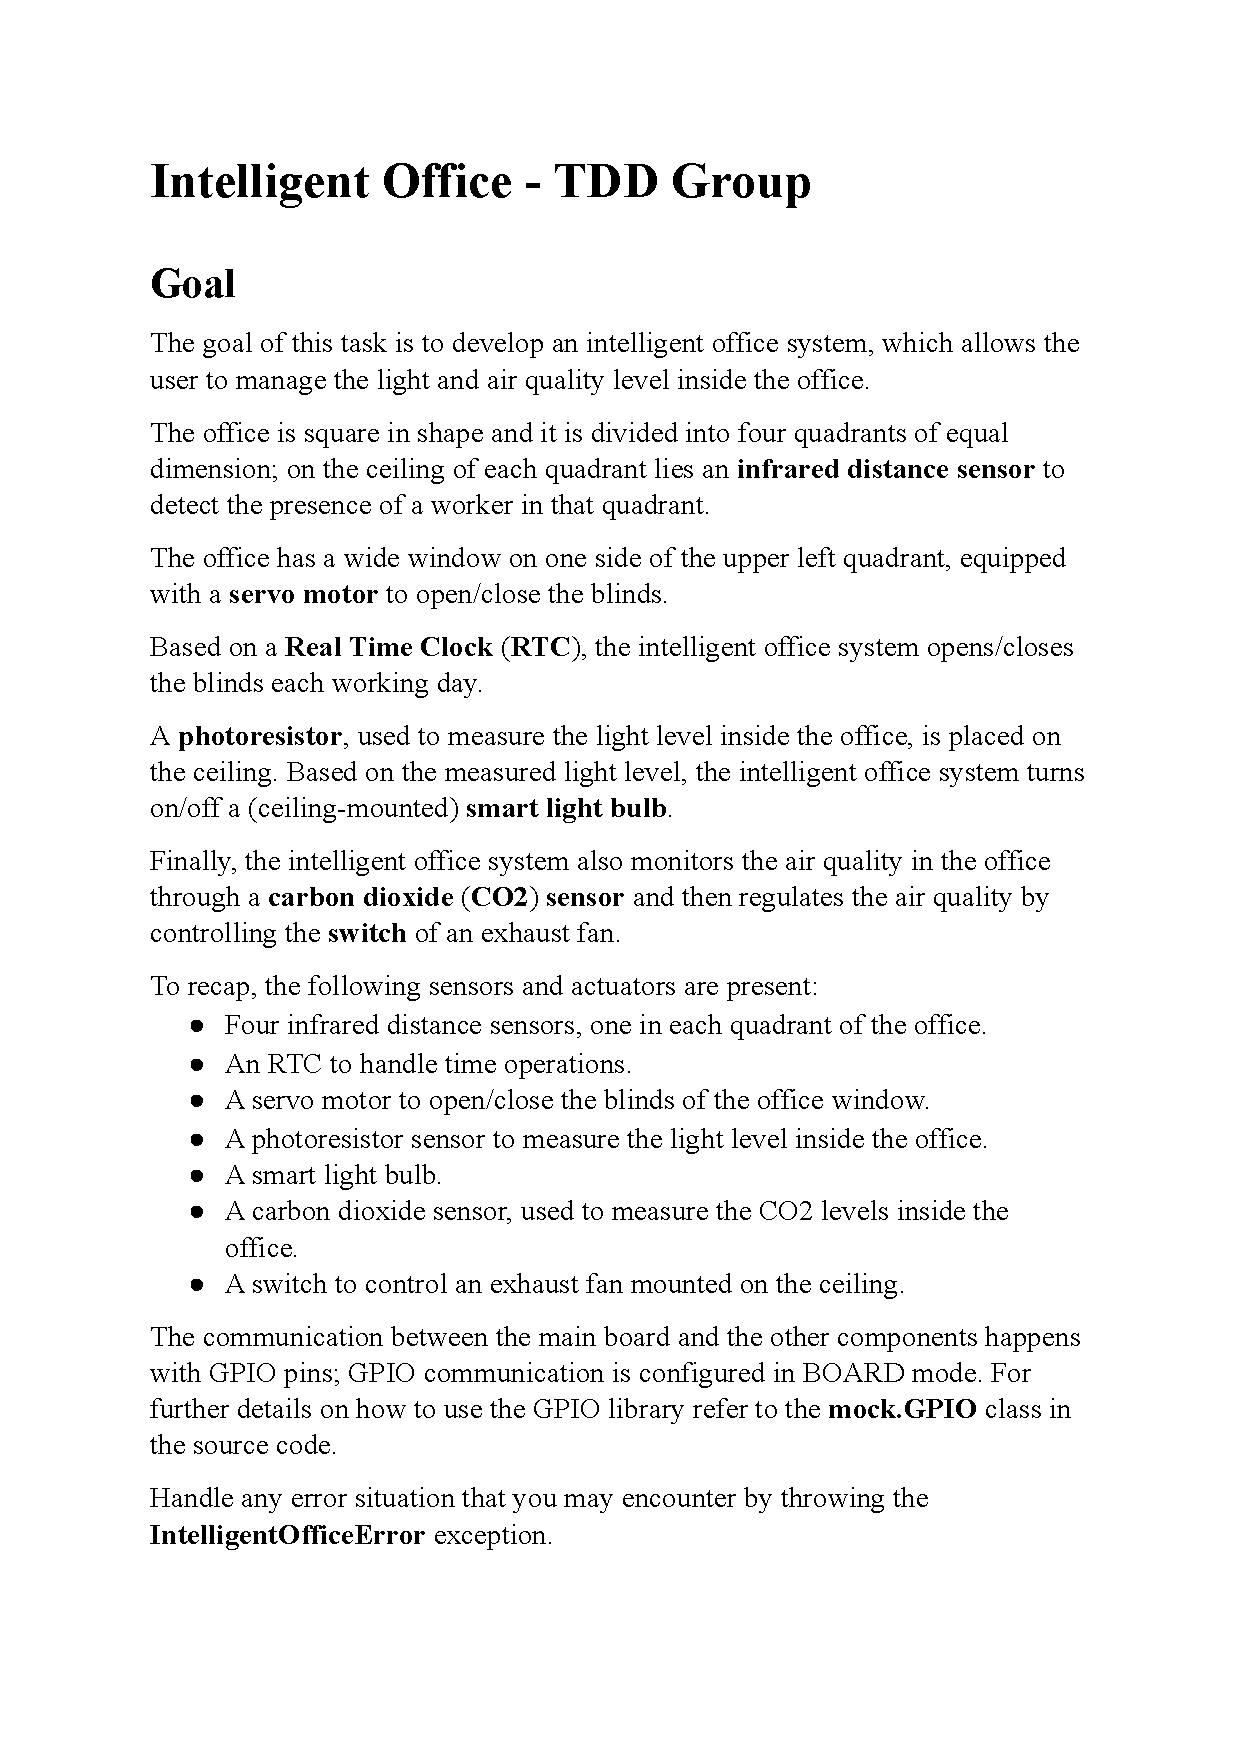
\includepdf[pages=-, pagecommand={}, linktodoc=true]{appendix/experimental_tasks/intelligent_office_tdd.pdf}
        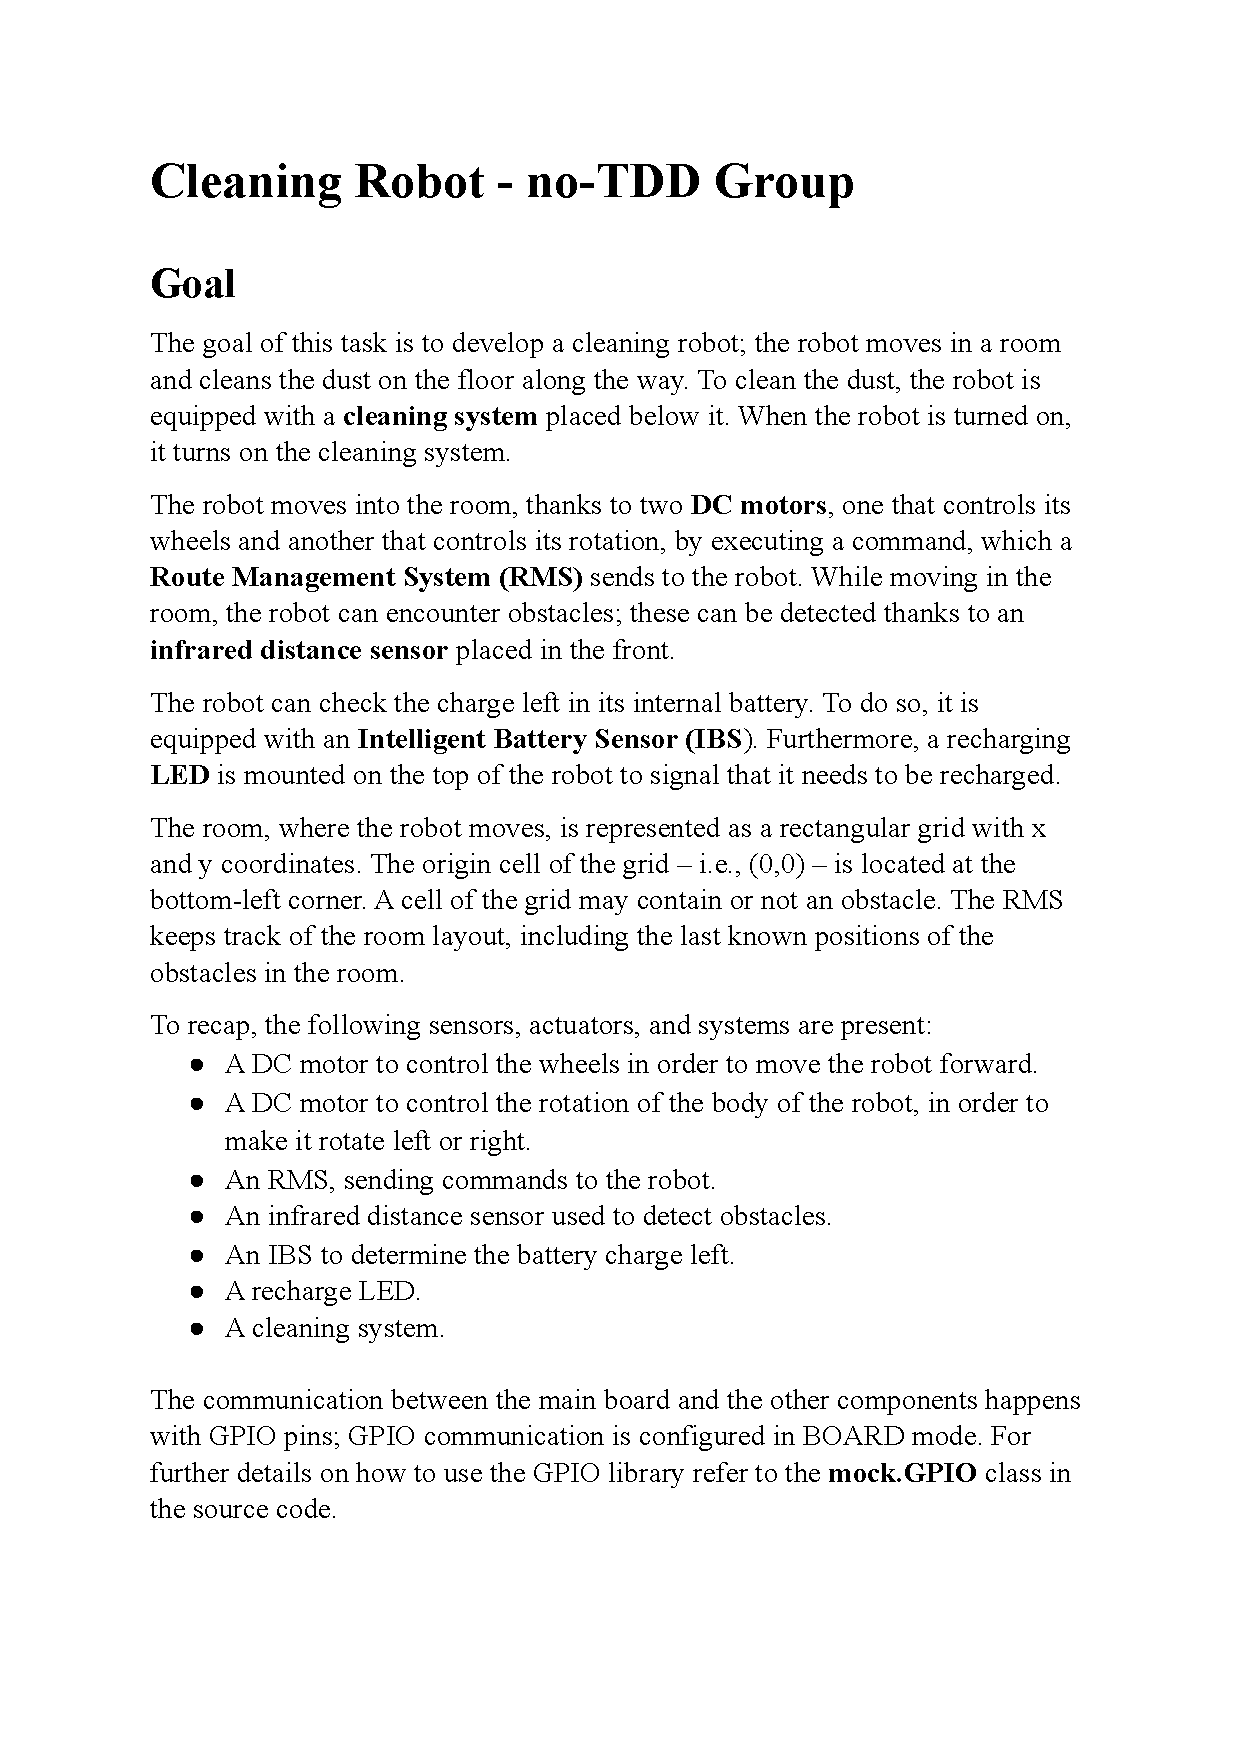
\includepdf[pages=-, pagecommand={}, linktodoc=true]{appendix/experimental_tasks/cleaning_robot_no_tdd.pdf}
        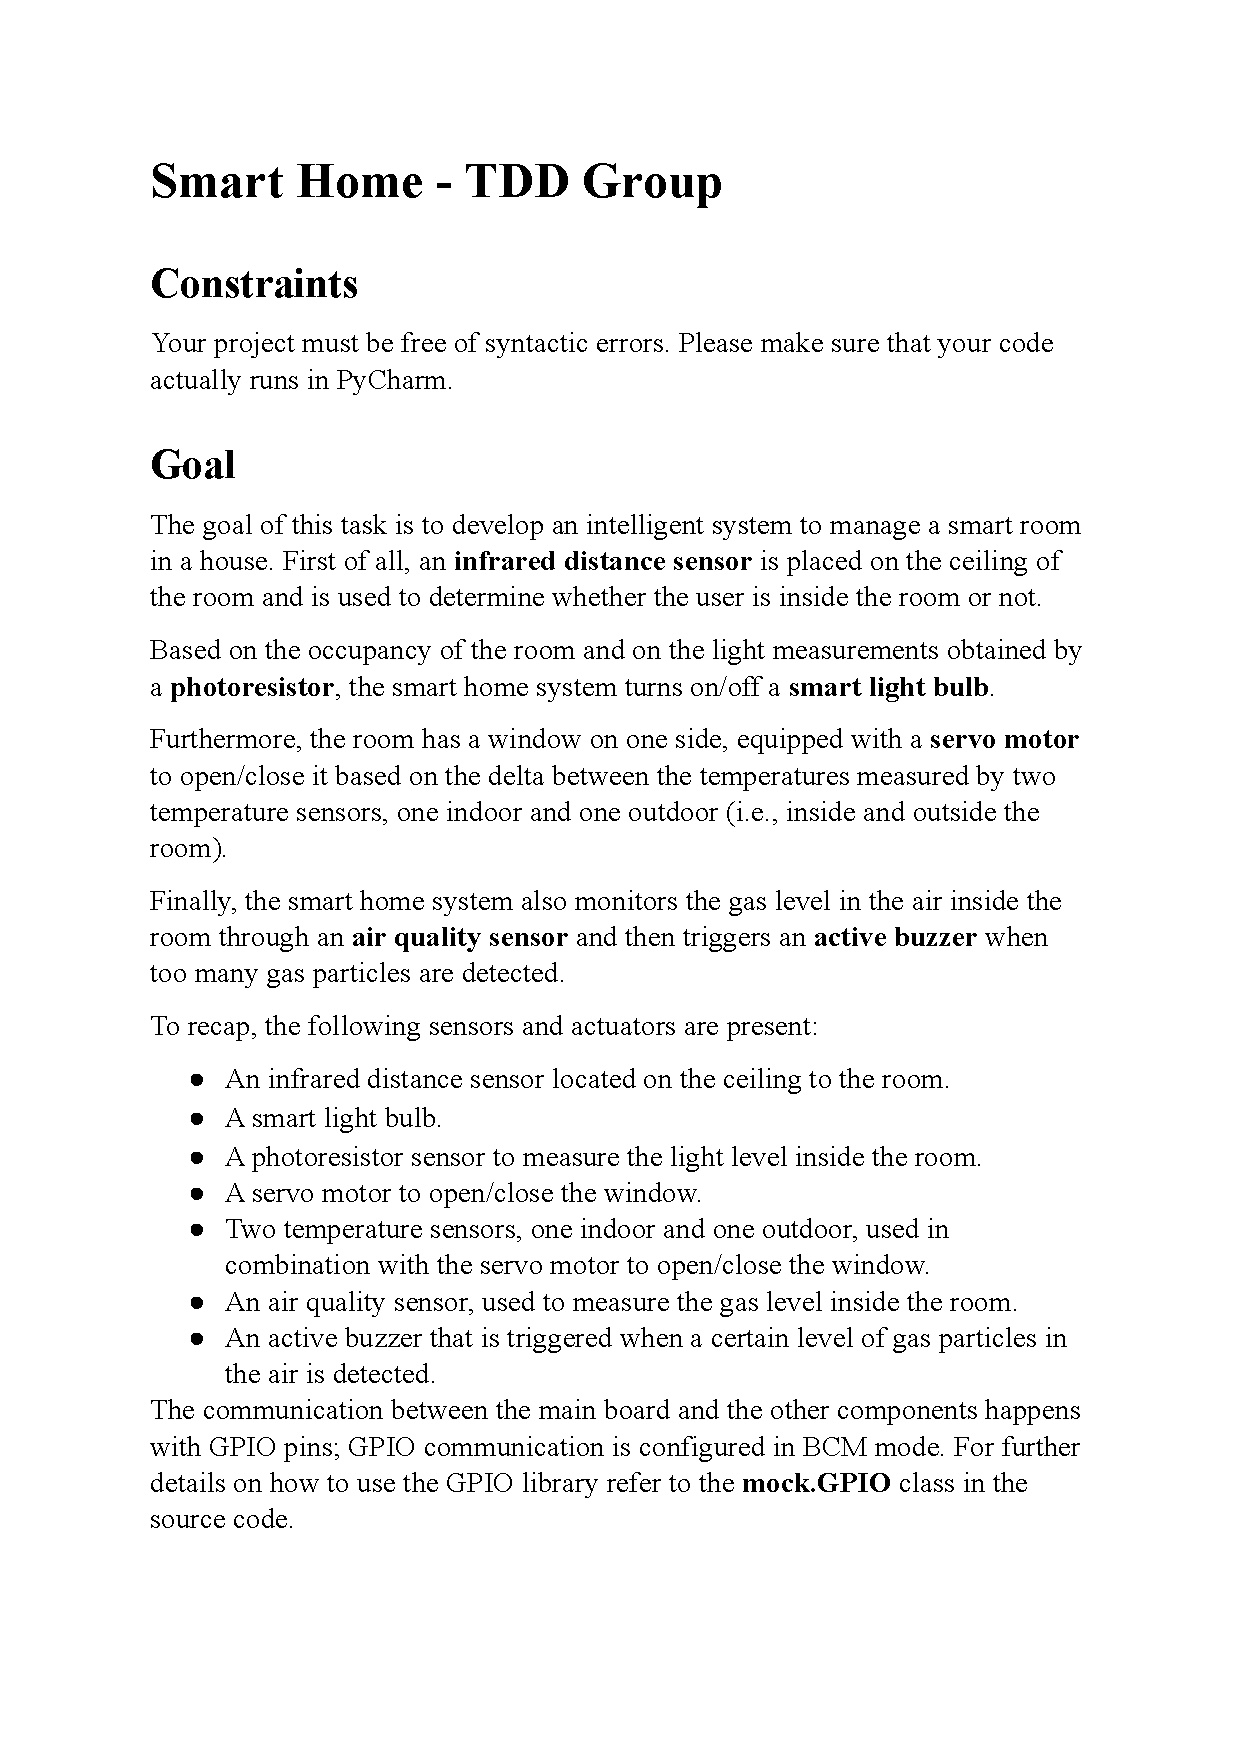
\includepdf[pages=-, pagecommand={}, linktodoc=true]{appendix/experimental_tasks/smart_home_tdd.pdf}
        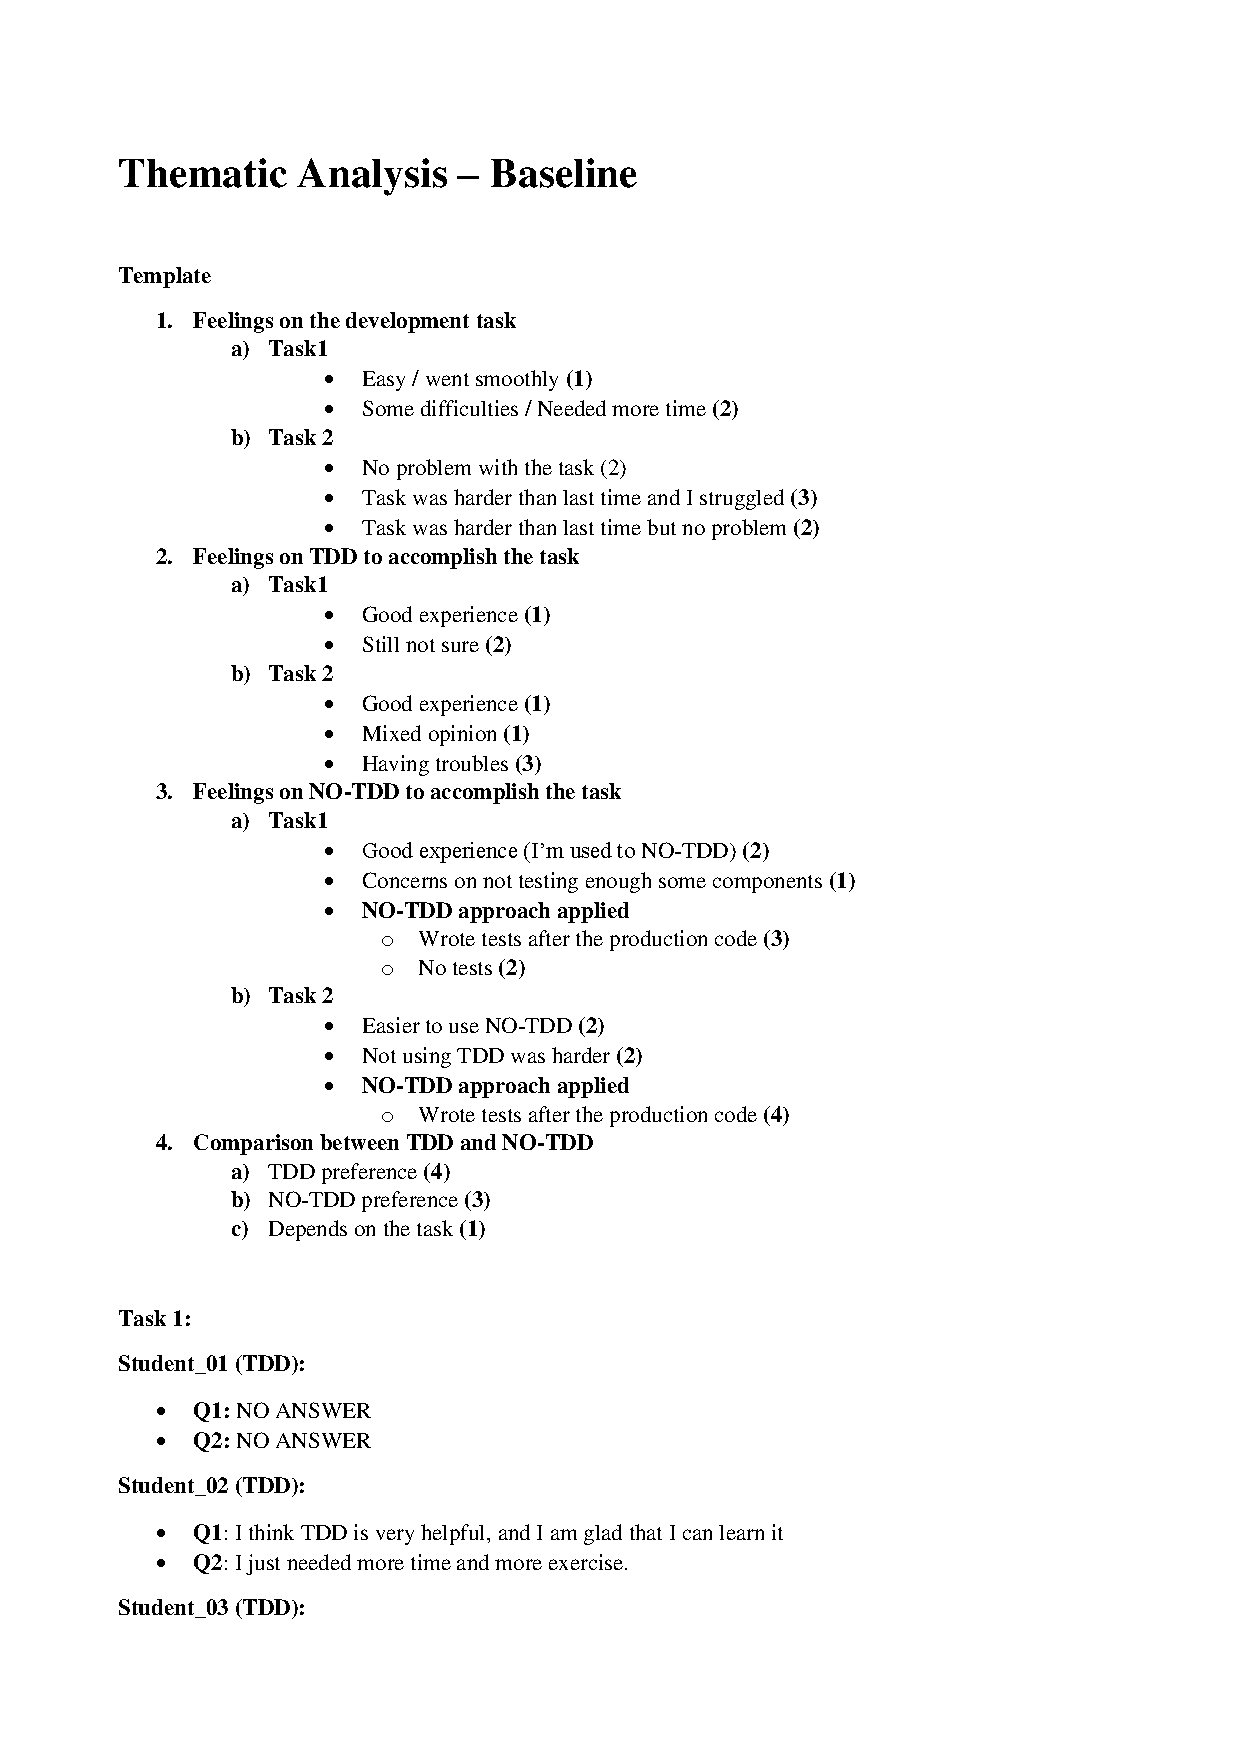
\includepdf[pages=-, pagecommand={}, linktodoc=true]{appendix/thematic_analysis/thematic_analysis_baseline.pdf}
        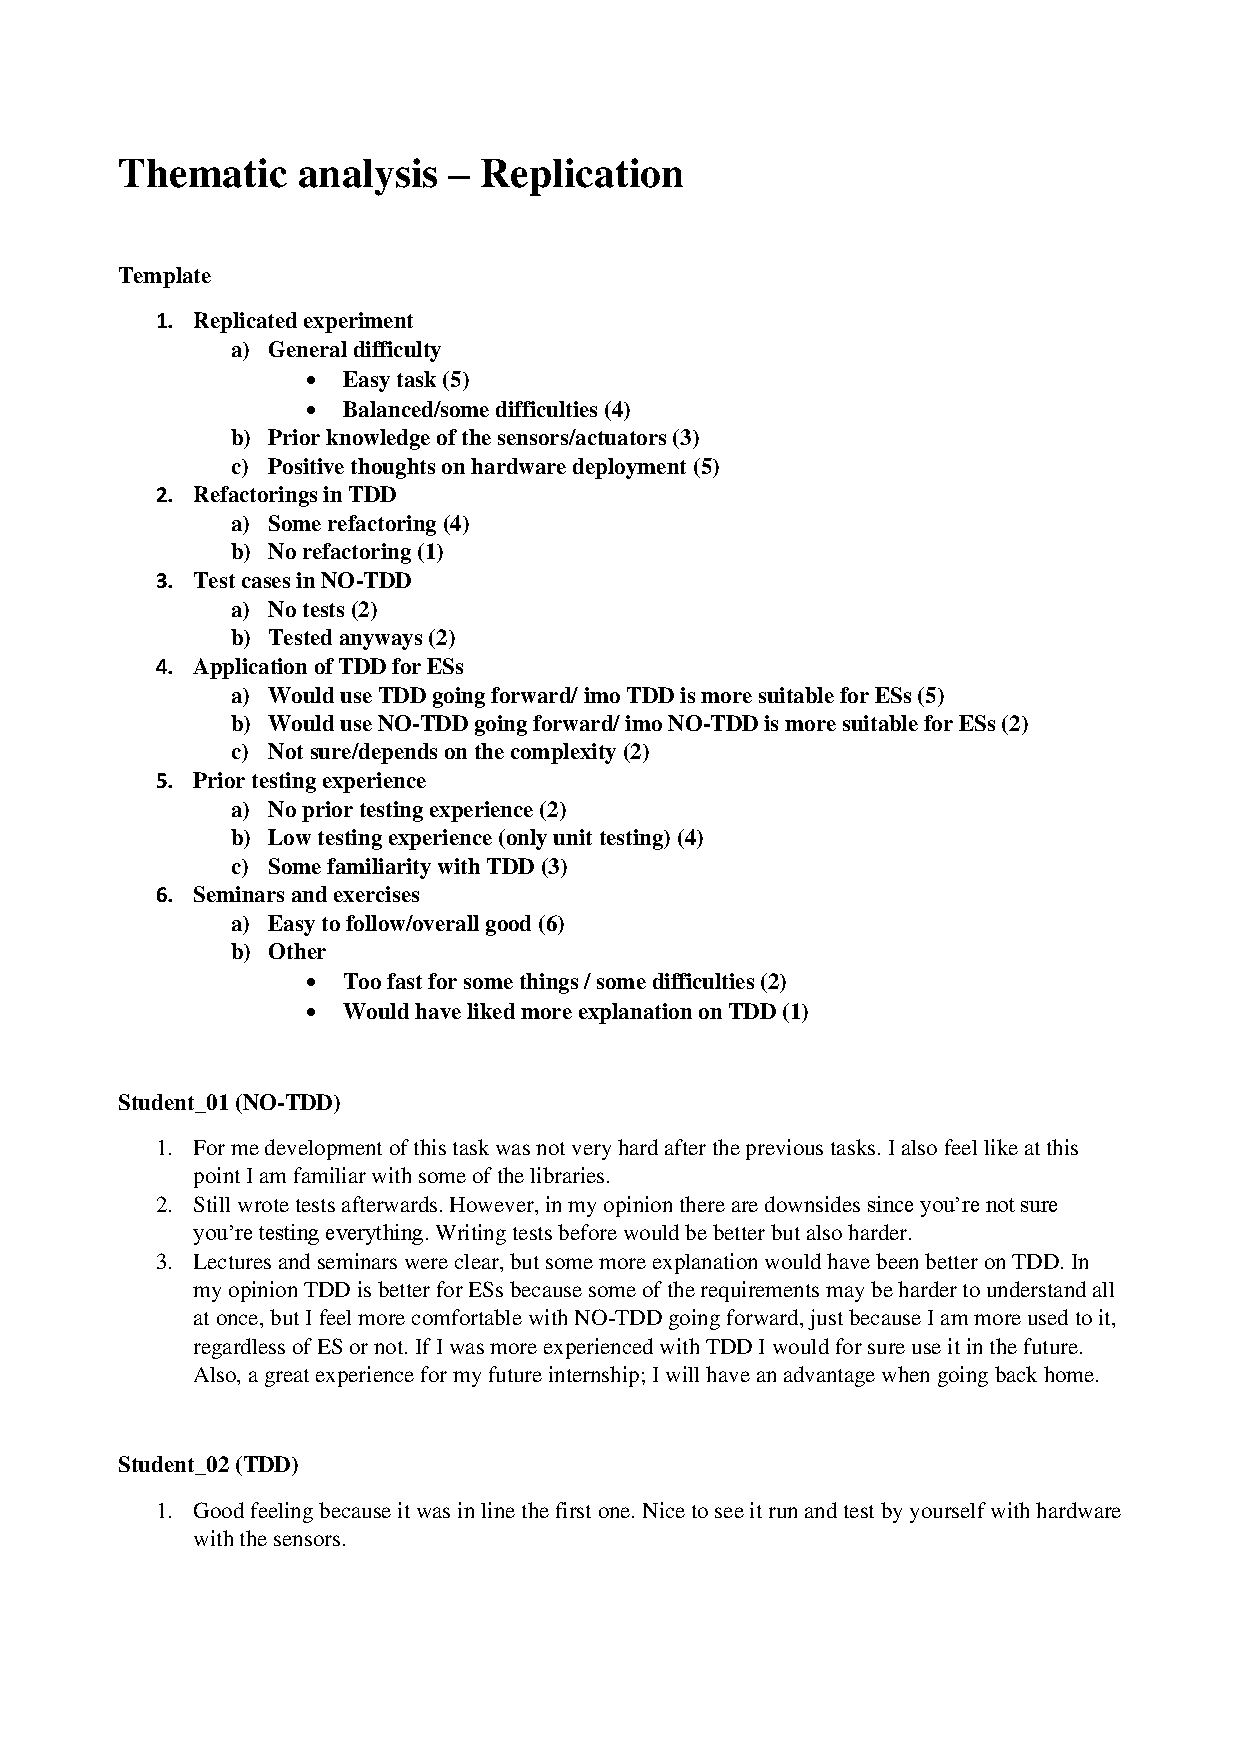
\includepdf[pages=-, pagecommand={}, linktodoc=true]{appendix/thematic_analysis/thematic_analysis_replication.pdf}
    \end{appendices}

\end{document}
